\newcommand{\bra}[1]{\langle #1|}
\newcommand{\ket}[1]{|#1\rangle}
\newcommand{\MET}{\slashed{E}_T}
\newcommand{\mDM}{m_{\rm{DM}}}
\newcommand{\mMed}{M_{\rm{med}}}
\newcommand{\gDM}{g_{\rm{DM}}}
\newcommand{\gq}{g_q}
\newcommand{\ifb}{\rm{fb}^{-1}}

\subsection{Vector and axial vector mediator, s-channel exchange}
\label{sec:monojet_V}

%\begin{itemize}
%\item Matrix Element implementations (with references)
%\begin{itemize}
% \item Production mechanism
% \item Lagrangian
% \item Definition of minimal width
%\end{itemize}
%\item Couplings
%\item Parameter choices (for scan)
%Vary mediator mass and DM mass 
%\item Generator implementation
%There are several matrix element implementations of the s-channel vector mediated DM production. This is available in POWHEG, MADGRAPH and also MCFM.
%The implementation in POWHEG generates DM pair production with 1 parton at Next-to-Leading-Order, whilst Madgraph and MCFM are at leading order. As shown in POWHEG paper{Haisch:2013ata}, including NLO corrections result in an enhancement in the cross section as compared to leading-order (LO) and though this is not significant, it does lead to a substantial reduction in the dependence on the choice of the renormalisation and factorisation scale and hence the theoretical uncertainty on the signal prediction. 
%Since NLO calculations are available for the process in POWHEG, we recommend to proceed with POWHEG as the generator of choice. 
%In addition to this, studies conducted within the DM forum have shown that POWHEG is more efficient for the generation of events all the way out to the tails of the kinematic distributions (https://indico.cern.ch/event/374678/session/0/material/3/1.pdf). 
%The input configuration in POWHEG allows you to set parameters to not generate events below a given $k{T}$ cut ('bornktmin') and an additional parameter that ensures sufficient statistics at high transverse momentum ('bornsuppfact). With these flags set to appropriate variables, it is then possible to use a single POWHEG sample to generate the Monte Carlo for all signal regions, whereas with Madgraph more individual samples to be stitched together to achieve the required statistics out to the tails of the kinematic distributions. 
%The POWHEG and Madgraph implementations were compared and the yields obtained from both were found to be compatible.  
%\end{itemize}

\begin{figure*}[t!]
\centering
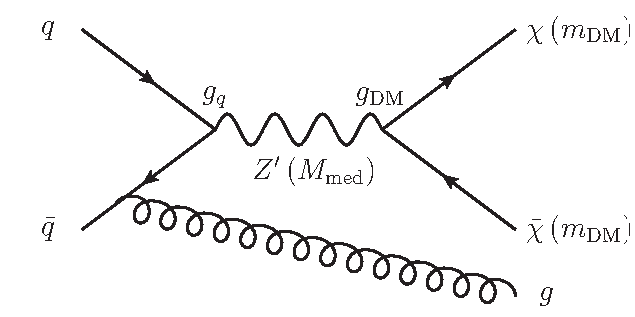
\includegraphics[width=0.5\linewidth]{figures/monoLHC.pdf}
\caption[][\baselineskip]{The diagram shows the pair production of dark matter particles in association with a parton from the initial state via an s-channel vector or axial-vector mediator. The process if specified by ($\mMed ,\, \mDM ,\, \gDM ,\, \gq)$, the mediator and dark matter masses, and the mediator couplings to dark matter and quarks respectively.}
\label{fig:OP}
\end{figure*}


There are several matrix element implementations of the s-channel vector mediated DM production. This is available in POWHEG, MADGRAPH and also MCFM.
The implementation in POWHEG generates DM pair production with 1 parton at next-to-leading order (NLO), whilst MADGRAPH and MCFM are at leading order (LO). As shown in POWHEG Ref.\,\cite{Haisch:2013ata}, including NLO corrections result in an enhancement in the cross section as compared to LO and though this is not significant, it does lead to a substantial reduction in the dependence on the choice of the renormalization and factorization scale and hence the theoretical uncertainty on the signal prediction. 
Since NLO calculations are available for the process in POWHEG, we recommend to proceed with POWHEG as the generator of choice. 




%Lagrangian
We consider the case of a dark matter particle that is a Dirac fermion and where the production proceeds via the exchange of a spin-1 $s$-channel mediator. We consider the following interactions between the DM and SM fields including a vector mediator with:\\
(a) vector couplings to DM and SM,\\
(b) axial-vector couplings to DM and SM.\\
\noindent The corresponding Lagrangians are
\begin{align}
\label{eq:AV} 
\mathcal{L}_{\mathrm{vector}} &= \sum_q \gq Z'_{\mu} \bar{q}\gamma^{\mu}q + \gDM Z'_{\mu} \bar{\chi}\gamma^{\mu}\chi \\
\mathcal{L}_{\rm{axial-vector}} &= \sum_q \gq Z'_{\mu} \bar{q}\gamma^{\mu}\gamma^5q + \gDM Z'_{\mu} \bar{\chi}\gamma^{\mu}\gamma^5\chi
\end{align}
where the coupling extends over all the quarks and universal couplings are assumed for all the quarks. 
It is also possible to consider another model in which mixed vector and axial-vector couplings are considered, for instance the couplings to the quarks are vector whereas those to DM are axial-vector. As a starting point, we consider only the models with the vector couplings only and axial vector couplings only.
%TODO Studies have been performed to see if the case of a mixed coupling can be simply extracted from the other models by some reweighting procedure to take account of the difference in cross section. This would assume that the difference between the pure and mixed couplings case does not affect the kinematics of the event. 


%Definition of minimal width
We assume that no additional visible or invisible decays contribute to the width of the mediator, this is referred to as the minimal width and it is defined as follows for the vector and axial-vector models.

\begin{equation}
%\Gamma_{\rm{min}}=\Gamma_{\bar{\chi}\chi} + \sum_{q}N_{c}\Gamma_{\bar{q}q}
\Gamma_{\rm{min}}=\Gamma_{\bar{\chi}\chi} + \sum_{q}\Gamma_{\bar{q}q}
\label{eq:monojet_min}
\end{equation}
where the individual contributions to this from the partial width are from

\begin{align}
\Gamma_{\bar{\chi}\chi}^{\rm{V}}&=\frac{\gDM^2 \mMed}{12\pi}\left(1+\frac{2 \mDM^2}{\mMed^2} \right)\sqrt{1-\frac{4 \mDM^2}{\mMed^2}}\\
\Gamma_{\bar{q}q}^{\rm{V}}&= \frac{3 \gq^2 \mMed}{12\pi}\left(1+\frac{2 m_q^2}{\mMed^2} \right)\sqrt{1-\frac{4 m_q^2}{\mMed^2}}\\
\Gamma_{\bar{\chi}\chi}^{\rm{A}}&=\frac{\gDM^2 \mMed}{12\pi} \left(1-\frac{4 \mDM^2}{\mMed^2}\right)^{3/2}\\
\Gamma_{\bar{q}q}^{\rm{A}}&= \frac{3 \gq^2 \mMed}{12\pi}\left(1-\frac{4 m_q^2}{\mMed^2}\right)^{3/2}\label{eq:Gamma4}\;.
\end{align}
Note the color factor 3 in the quark terms.
Figure\,\ref{fig:monojet_width_V} shows the minimal width as a function of mediator mass for both vector and axial-vector mediators assuming couplings of 1. With this choice of the couplings, the dominant contribution to the minimal width comes from the quarks due to the color factor enhancement.

\begin{figure}
\centering
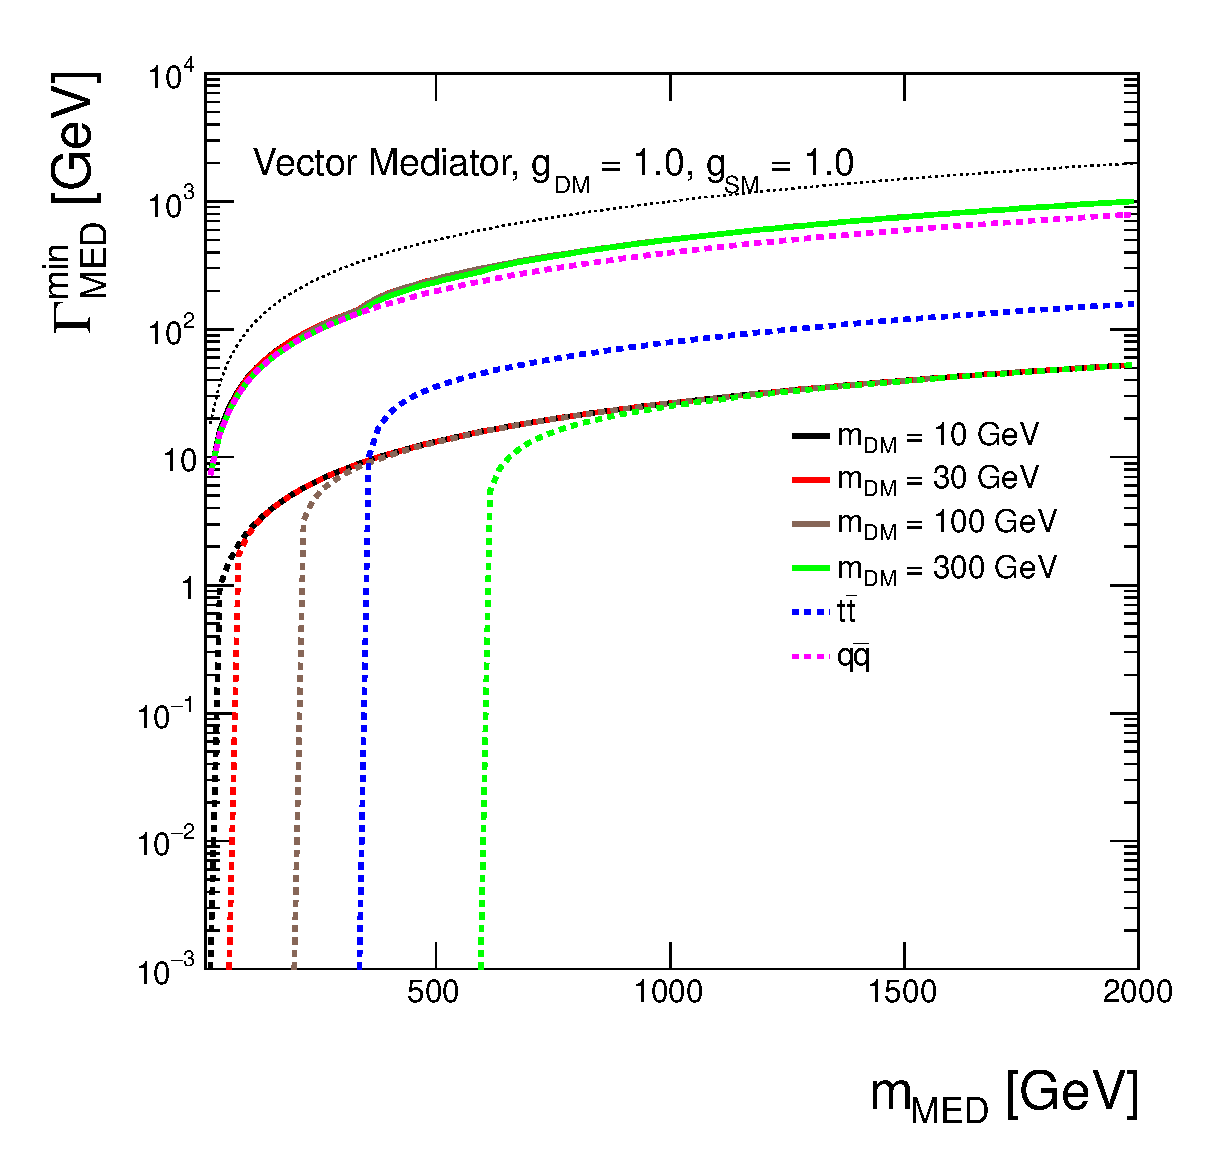
\includegraphics[width=0.45\linewidth]{figures/monojet/width_V.eps}
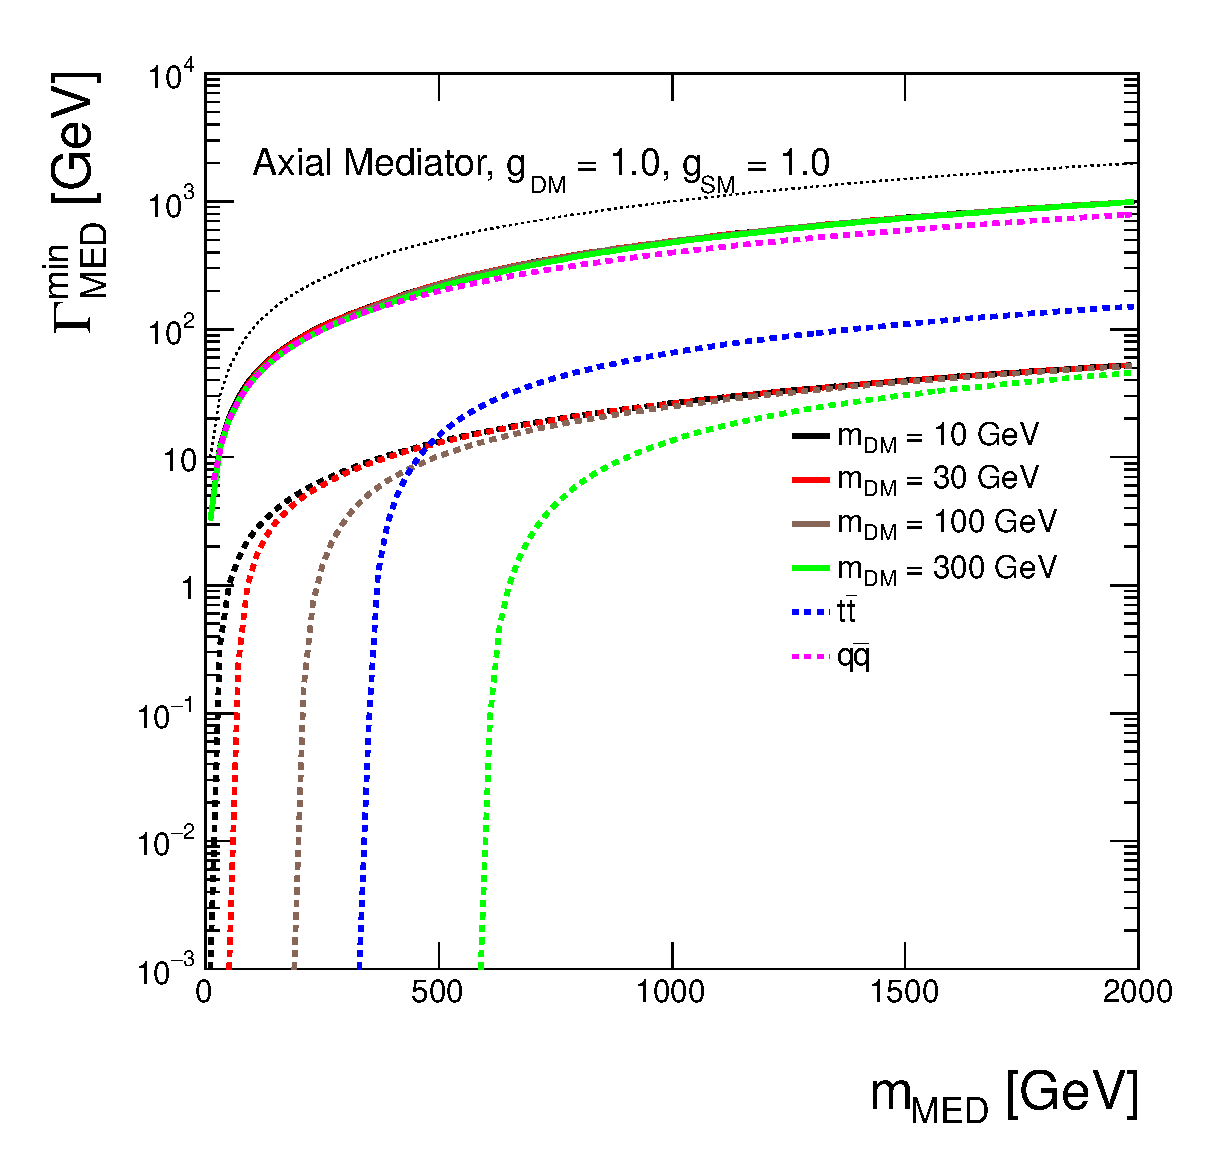
\includegraphics[width=0.45\linewidth]{figures/monojet/width_A.eps}
\caption{Minimal width as a function of mediator mass for vector and axial-vector mediator assuming couplings of 1. The total width is shown as solid lines for Dark Matter masses of 10\,GeV, 30\,GeV, 100\,GeV and 300\,GeV in black, red, brown and green, respectively. The individual contributions from Dark Matter are indicated by dotted lines with the same colors. The contribution from all quarks but top is shown as magenta dotted line and the contribution from top quarks only is illustrated by the dotted blue line. The dotted black line shows the extreme case $\Gamma_{\rm{min}}=\mMed$.}
\label{fig:monojet_width_V}
\end{figure}

The simplified models described here have four free parameters: mediator mass $\mMed$, Dark Matter mass $\mDM$, coupling of the mediator to quarks $g_q$ and coupling of the mediator to Dark Matter $\gDM$. In order to determine an optimal choice of the parameter grid for presentation of the early Run-2 results, dependencies of the kinematic quantities and cross sections on the individual parameters need to be studied. The following paragraphs list the main observations from the scans over the parameters that support the final proposal for the parameter grid.


\paragraph{Scan over the couplings}

Figure\,\ref{fig:monojet_scan_V_g} reveals there are no differences in the shape of the $\MET$ distribution among the samples where the pair of 10\,GeV Dark Matter particles are produced on-shell from the mediator of 1\,TeV, generated with different choice of the coupling strength. The considered coupling values range from 0.1 to 1.45, where the latter value approximates the maximum allowed coupling value, holding $g_q=\gDM$, such that $\Gamma_{\rm{min}} < \mMed$.
Based on similar plots for different choices of mediator and Dark Matter masses, it is concluded that the shapes of kinematic distributions are not altered neither for the on-shell Dark Matter production where $\mMed>2\mDM$, nor for the off-shell Dark Matter production where $\mMed<2\mDM$. Only the cross sections change.
Differences in kinematic distributions are expected only close to the transition region where both on-shell and off-shell regimes mix.
%TODO clarify slide 9 and 10 in https://indico.cern.ch/event/389275/contribution/1/material/slides/0.pdf
%TODO check explicitly for V and A (generate corresponding samples)
\begin{figure}
\centering
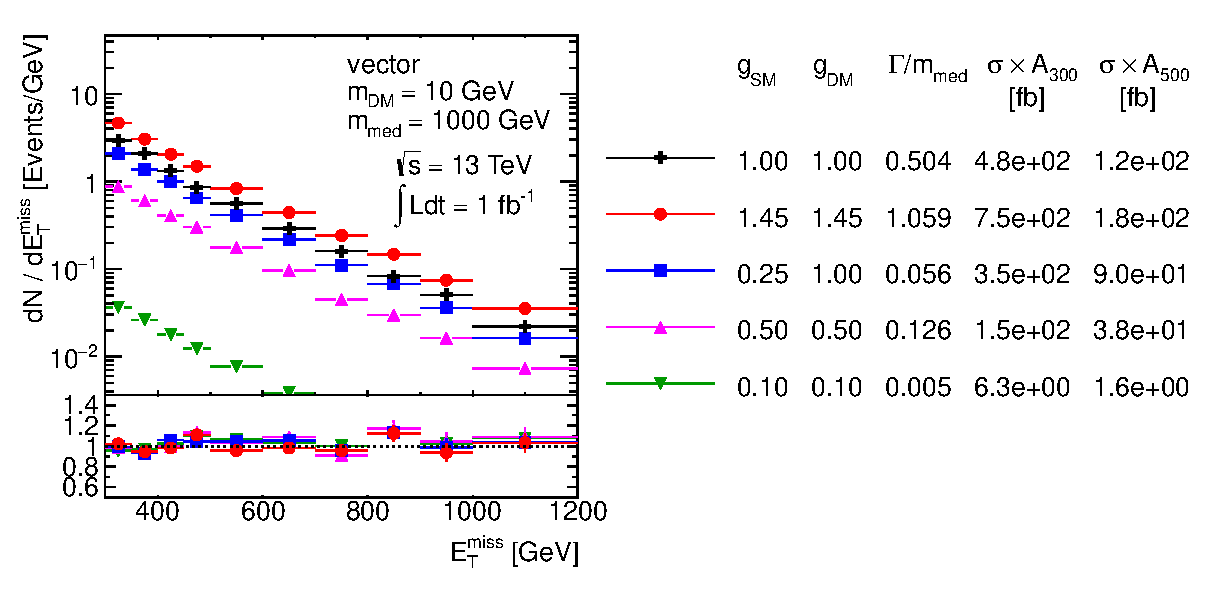
\includegraphics[width=0.9\linewidth]{figures/monojet/scan_g_V_10_1000.eps}
\caption{Scan over couplings. The $\MET$ distribution is compared for the vector mediator models using the parameters as indicated. Ratios of the normalized distributions with respect to the first one are shown. $A_{300}$ and $A_{500}$ in the table denote the acceptance of the $\MET>300$\,GeV and $\MET>500$\,GeV cut, respectively.}
\label{fig:monojet_scan_V_g}
\end{figure}

The only place where special care needs to be taken are extremely heavy and narrow mediators, in other words with low couplings. Figure\,\ref{fig:monojet_narrow} suggests a change in the shape of the $\MET$ distribution for 5\,TeV mediator once $\Gamma_{\rm{min}}/\mMed$ gets down to the order of percent or below.
This, however, does not come from physics as it is a feature of the generator implementation, where a cutoff for the regions far away from the mediator mass is often used. This is illustrated in Fig.\,\ref{fig:monojet_mchichi} showing the invariant mass of the Dark Matter pair in the samples generated for 7\,TeV mediator with different coupling strength. In all cases, it is expected to observe a peak around the mediator mass with a tail extending to $m_{\bar{\chi}\chi}\rightarrow0$, significantly enhanced by parton distribution functions at low Bjorken $x$. For coupling strength 1 and 3, the massive enhancement at $m_{\bar{\chi}\chi}\rightarrow0$ implies the resonant production at $m_{\bar{\chi}\chi}=7$\,TeV is statistically suppressed such that barely any events are generated there. However, for narrower mediators with couplings below 1, the peak around 7\,TeV is clearly visible in the generated sample and the dominant tail at $m_{\bar{\chi}\chi}\rightarrow0$ is artificially cut off, leading to unphysical cross section predictions and kinematic shapes. This explains why the sample with the narrowest mediator in Fig.\,\ref{fig:monojet_narrow} is heavily suppressed in terms of production cross section and also gives different $\MET$ shape.
In general, for such extreme parameter choices
%as $\mMed=7$\,TeV and $\Gamma_{\rm{min}}=36$\,GeV,
the EFT model should give the correct answer. In case the simplified model calculation does not reproduce the EFT result, the phase space generation of the simplified model has to be carefully examined in order to understand the cause of the problem. Fortunately, this is a rather academic discussion as such extreme corners of the parameter space are not going to be considered for presentation of Run-2 results.

%Uli: as fabio says, increasing bwcutoff might improve things in the case you are considering
%
%for a mediator with mass M = 7 TeV and width Gamma = 36 GeV, i think the correct way to do this calculation is to work in an EFT; this should give you the correct result
%
%in fact, if your simplified model calculation does not reproduce the EFT result for such extreme parameter choices, you have to carefully look at the phase-space generation of the simplified model calculation (as you did). at the end you probably have to tailor the phase-space generator of madgraph, powheg, etc. to get it right; this will be non-trivial since phase-space generation is an art! furthermore, one has to do this process 
%by process and the difficulties will increase from mono-jet to ttbar + MET, etc. 

\begin{figure}
\centering
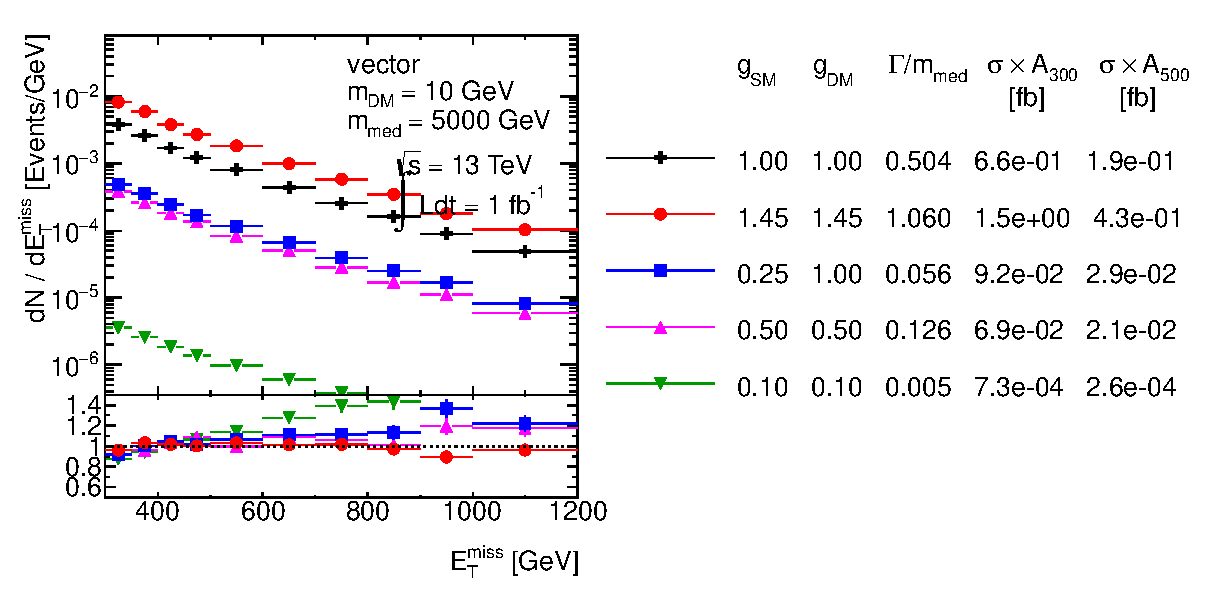
\includegraphics[width=0.9\linewidth]{figures/monojet/scan_g_V_10_5000.eps}
\caption{Scan over couplings. The $\MET$ distribution is compared for the vector mediator models using the parameters as indicated. Ratios of the normalized distributions with respect to the first one are shown. $A_{300}$ and $A_{500}$ in the table denote the acceptance of the $\MET>300$\,GeV and $\MET>500$\,GeV cut, respectively.}
\label{fig:monojet_narrow}
\end{figure}

\begin{figure}
\centering
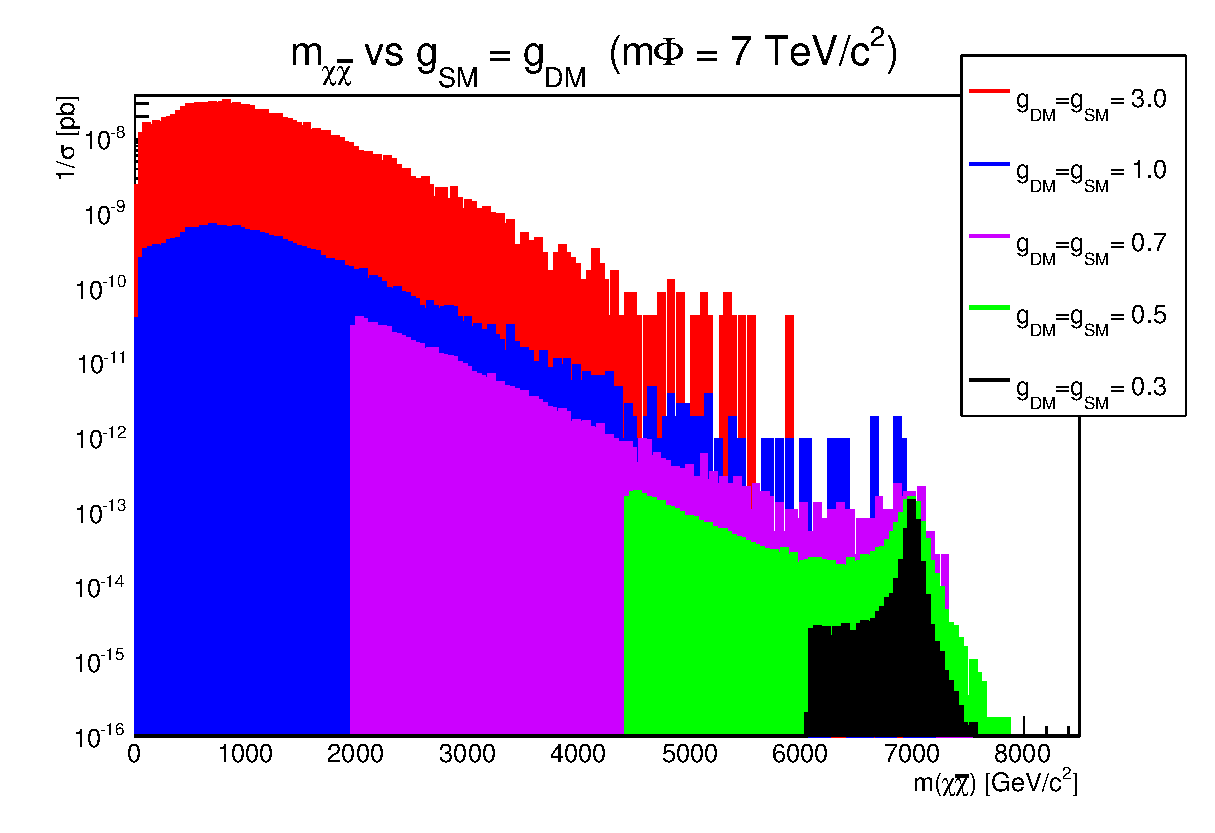
\includegraphics[width=0.9\linewidth]{figures/monojet/mphi_vs_g_xsecwgt_7tev.eps}
\caption{Invariant mass of the Dark Matter pair in the samples with $\mMed=7$\,TeV and different coupling strengths.}
\label{fig:monojet_mchichi}
\end{figure}

\paragraph{Scan over the Dark Matter mass}

For the fixed mediator mass and couplings, both the cross section and the kinematic distributions remain similar for different Dark Matter masses as long as $\mMed>2\mDM$. This is illustrated in Fig.\,\ref{fig:monojet_scan_V_mDM1000} on an example of 1\,TeV mediator and Dark Matter mases ranging from 10\,GeV to 300\,GeV. It is observed that the cross section decreases as the Dark Matter mass reaches closer to $\mMed/2$. Once the Dark Matter pair is produced off-line, the cross section of such simplified model is suppressed and the $\MET$ spectrum hardens, as demonstrated with the choice of 1\,TeV Dark Matter in the same plot. Figure\,\ref{fig:monojet_scan_V_mDM100} reveals the $\MET$ spectrum hardens further with increasing Dark Matter mass, accompanied by the gradual decrease of the cross section. From these observations one can conclude:
\begin{itemize}
\item A coarse binning along $\mDM$ is sufficient at $\mMed \gg 2\mDM$.
\item Finer binning is needed in order to capture the changes in the cross section and kinematic quantities close to the production threshold on both sides around $\mMed=2\mDM$.
\item Due to the significant cross section suppression of the off-shell Dark Matter pair production, it is not necessary to populate the parameter space $\mMed \ll 2\mDM$ since the LHC is not going to be able to probe the models there.
\end{itemize}

\begin{figure}
\centering
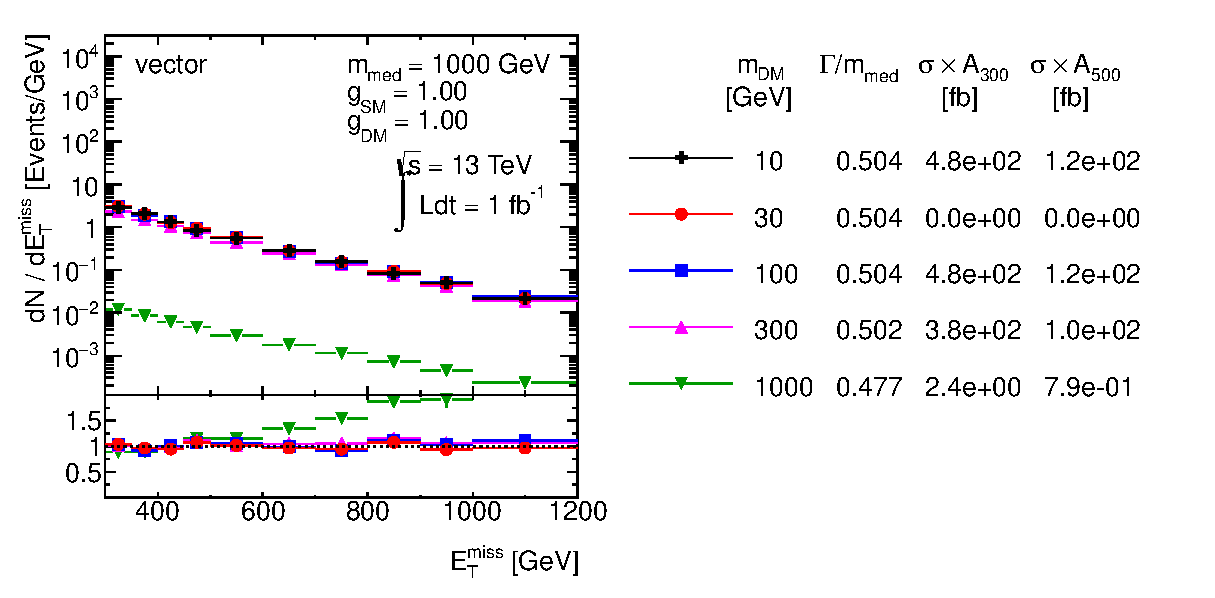
\includegraphics[width=0.9\linewidth]{figures/monojet/scan_mDM_V_1000.eps}
\caption{Scan over Dark Matter mass. The $\MET$ distribution is compared for the vector mediator models using the parameters as indicated. Ratios of the normalized distributions with respect to the first one are shown. $A_{300}$ and $A_{500}$ in the table denote the acceptance of the $\MET>300$\,GeV and $\MET>500$\,GeV cut, respectively.}
\label{fig:monojet_scan_V_mDM1000}
\end{figure}

\begin{figure}
\centering
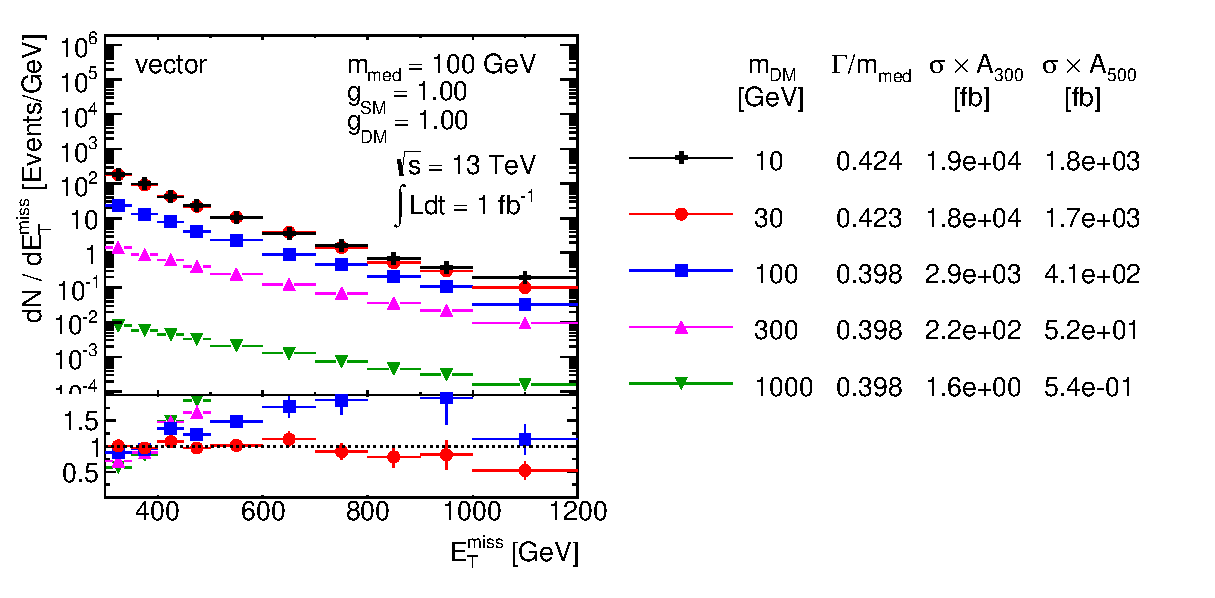
\includegraphics[width=0.9\linewidth]{figures/monojet/scan_mDM_V_100.eps}
\caption{Scan over Dark Matter mass. The $\MET$ distribution is compared for the vector mediator models using the parameters as indicated. Ratios of the normalized distributions with respect to the first one are shown. $A_{300}$ and $A_{500}$ in the table denote the acceptance of the $\MET>300$\,GeV and $\MET>500$\,GeV cut, respectively.}
\label{fig:monojet_scan_V_mDM100}
\end{figure}


\paragraph{Scan over the mediator mass}

Changing the mediator mass for fixed Dark Matter mass and couplings leads to significant differences in cross section and shapes of the kinematic variables for $\mMed>2\mDM$ as shown in Fig.\,\ref{fig:monojet_scan_V_mMed10}. As expected, higher mediator masses lead to harder $\MET$ spectra.
On the other hand, the $\MET$ shapes are similar in the off-shell Dark Matter production regime as well as no dramatic differences in cross sections are observed, which is illustrated in Fig.\,\ref{fig:monojet_scan_V_mMed1000}. Therefore, a coarse binning along $\mDM$ is sufficient at $\mMed \ll 2\mDM$.

\begin{figure}
\centering
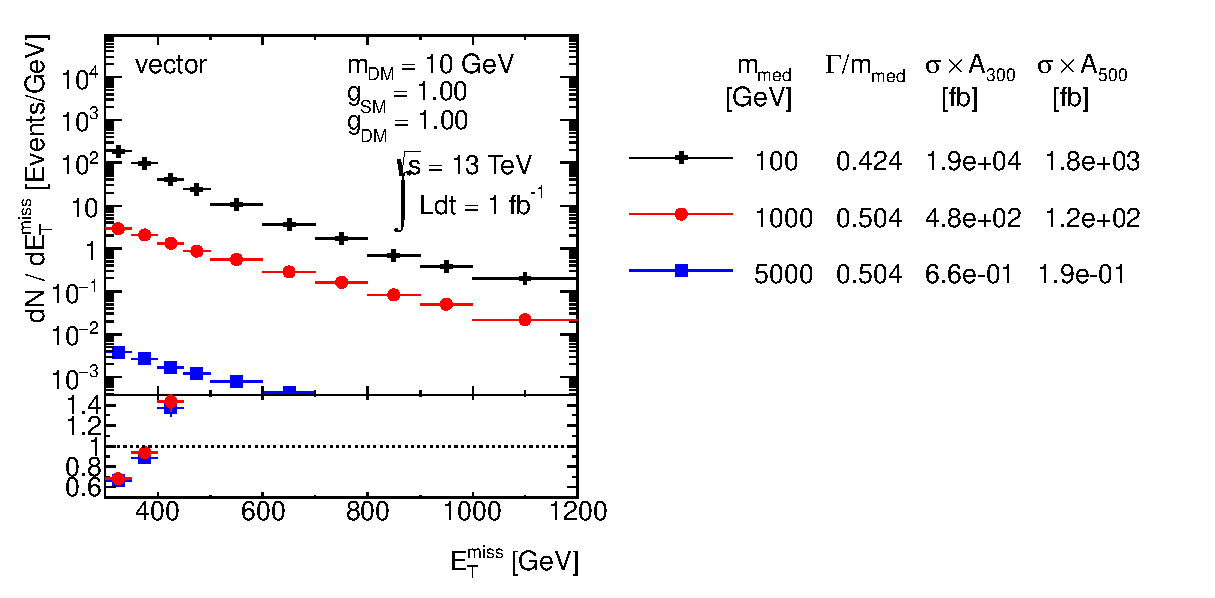
\includegraphics[width=0.9\linewidth]{figures/monojet/scan_mMed_V_10.eps}
\caption{Scan over mediator mass. The $\MET$ distribution is compared for the vector mediator models using the parameters as indicated. Ratios of the normalized distributions with respect to the first one are shown. $A_{300}$ and $A_{500}$ in the table denote the acceptance of the $\MET>300$\,GeV and $\MET>500$\,GeV cut, respectively.}
\label{fig:monojet_scan_V_mMed10}
\end{figure}

\begin{figure}
\centering
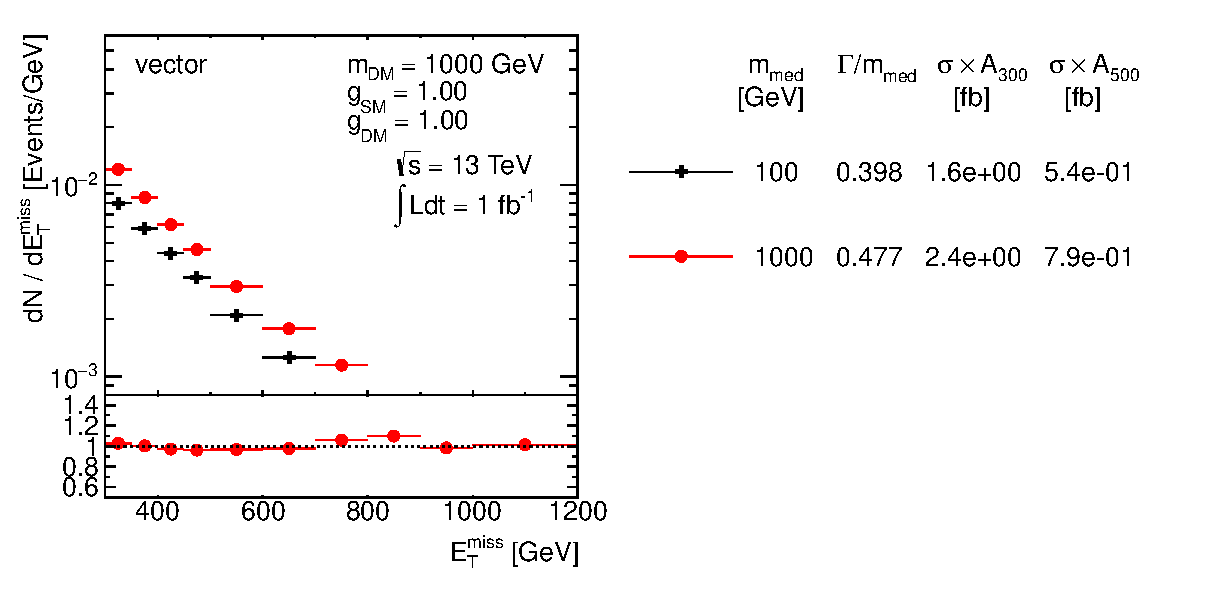
\includegraphics[width=0.9\linewidth]{figures/monojet/scan_mMed_V_1000.eps}
\caption{Scan over mediator mass. The $\MET$ distribution is compared for the vector mediator models using the parameters as indicated. Ratios of the normalized distributions with respect to the first one are shown. $A_{300}$ and $A_{500}$ in the table denote the acceptance of the $\MET>300$\,GeV and $\MET>500$\,GeV cut, respectively.}
\label{fig:monojet_scan_V_mMed1000}
\end{figure}


\paragraph{Proposed parameter grid}

Based on the observations above, the following proposal is made for the presentation of the early Run-2 results from the LHC:\\
(a) Give results in the $\mMed$--$\mDM$ plane for a particular choice of the couplings.\\
(b) Give results in the $g_q$--$\gDM$ plane for a particular choice of the masses.

%discuss expected sensitivity (cite PUB note) when motivating mDM and mMed range
%motivate the mass point for the coupilng scan

We choose to display the results in the $\mMed$--$\mDM$ plane for the choice of the couplings $g_q=\gDM=1$. In order to motivate the highest mediator mass grid point, the expected sensitivity of Run-2 LHC data needs to be taken into account.
The expected upper limit at 95\% confidence level on the product of cross section, acceptance and efficiency, $\sigma\times A\times\epsilon$, in the final Run-1 ATLAS mono-jet anaylsis\,\cite{Aad:2015zva} is 51\,fb and 7.2\,fb  for $\MET>300$\,GeV and $\MET>500$\,GeV, respectively. The ATLAS 14\,TeV prospects\,\cite{ATL-PHYS-PUB-2014-007} predict twice better sensitivity with the first $5\,\ifb$ of data already. Given the cross section for $V+$jets processes increases by roughly factor 2 %TODO this is just my guess, can we get more precise number and a citation?
when going from $\sqrt{s}=8$\,TeV to 13\,TeV, similar fiducial cross section limits can be expected with the first Run-2 data as from the final Run-1 analysis.
The generator level cross section times the acceptance at $\MET>500$\,GeV for the model with couplings $g_q=\gDM=1$, light Dark Matter of 10\,GeV and 1\,TeV vector mediator is at the order of 100\,fb, i.e. the early Run-2 mono-jet analysis is going to be sensitive to heavier mediators than this. The value of $\sigma\times A$ at $\MET>500$\,GeV for 5\,TeV vector mediator is at the order of 0.1\,fb, therefore this model probably lies beyond the reach of the LHC.
Based on these arguments, the following $\mMed$ grid points are chosen, equidistant in the logarithmic scale: 10\,GeV, 30\,GeV, 100\,GeV, 300\,GeV, 1000\,GeV and 3000\,GeV. Given the fact that significant changes in cross section happen around the $\mMed=2\mDM$ threshold, the $\mDM$ grid points are taken at $\mMed/2$, namely: 5\,GeV, 15\,GeV, 50\,GeV, 150\,GeV, 500\,GeV and 1500\,GeV.
The detailed studies of the impact of the parameter changes on the cross section and kinematic distributions presented earlier in this section support removing some of the grid points and rely on interpolation. The optimised grids proposed for the vector and axial-vector mediators are given in Fig.\,\ref{fig:monojet_grid_V}, containing 24 mass points each.
%mDM =    5  : mMed =   10    30   100   300  1000  3000  
%mDM =   15  : mMed =   10    30   100                    
%mDM =   50  : mMed =   10    30   100   300              
%mDM =  150  : mMed =   10         100   300  1000        
%mDM =  500  : mMed =   10               300  1000  3000
%mDM = 1500  : mMed =   10                    1000  3000

\begin{figure}
\centering
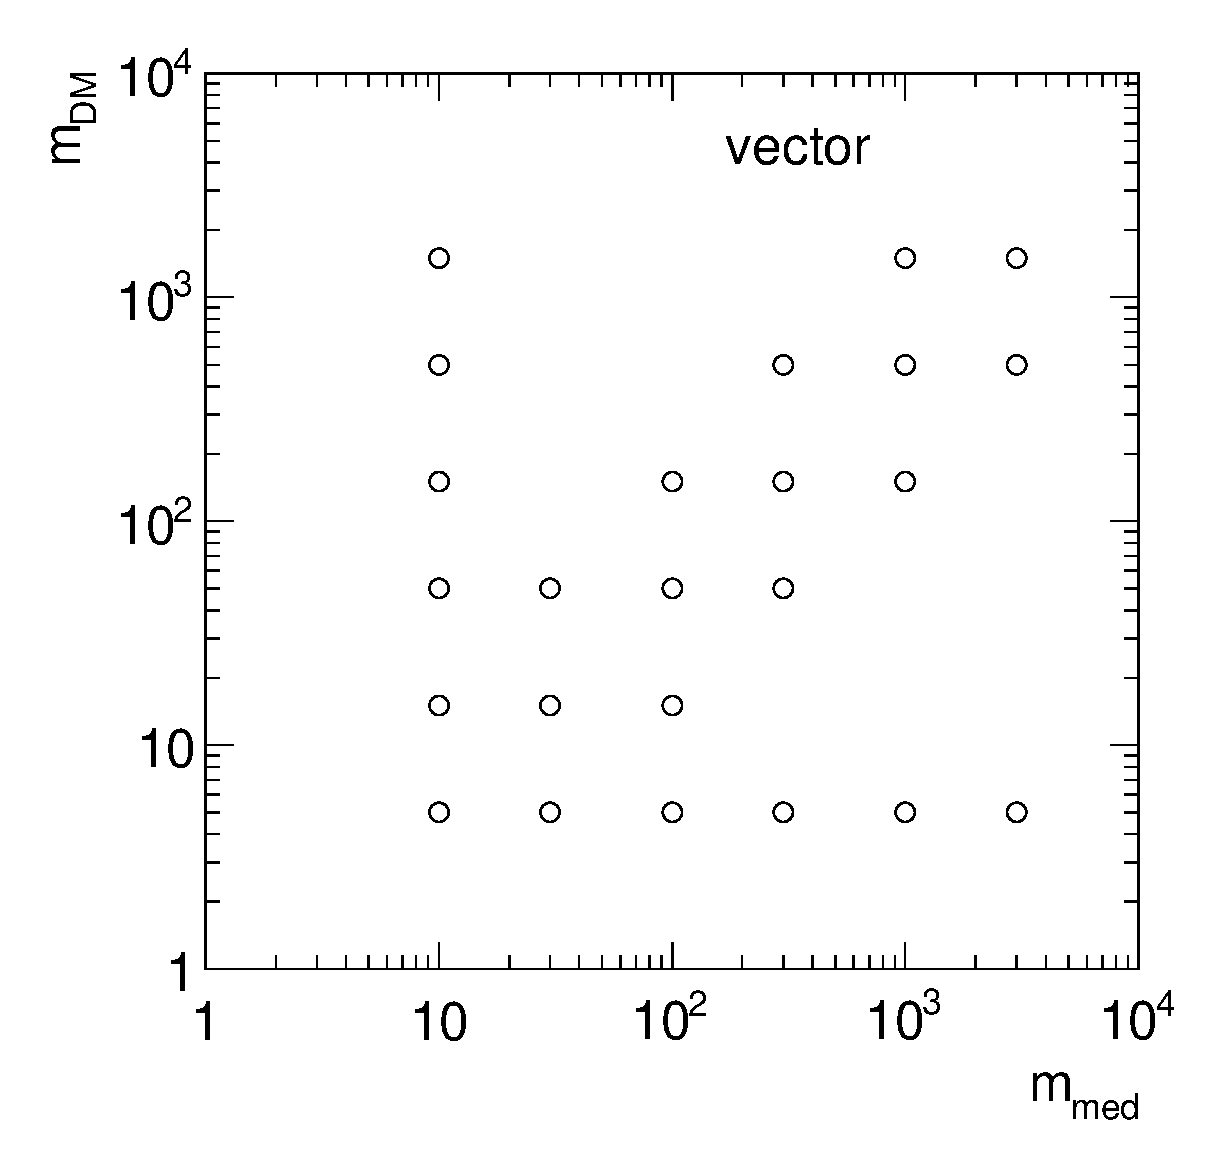
\includegraphics[width=0.45\linewidth]{figures/monojet/grid_V.eps}
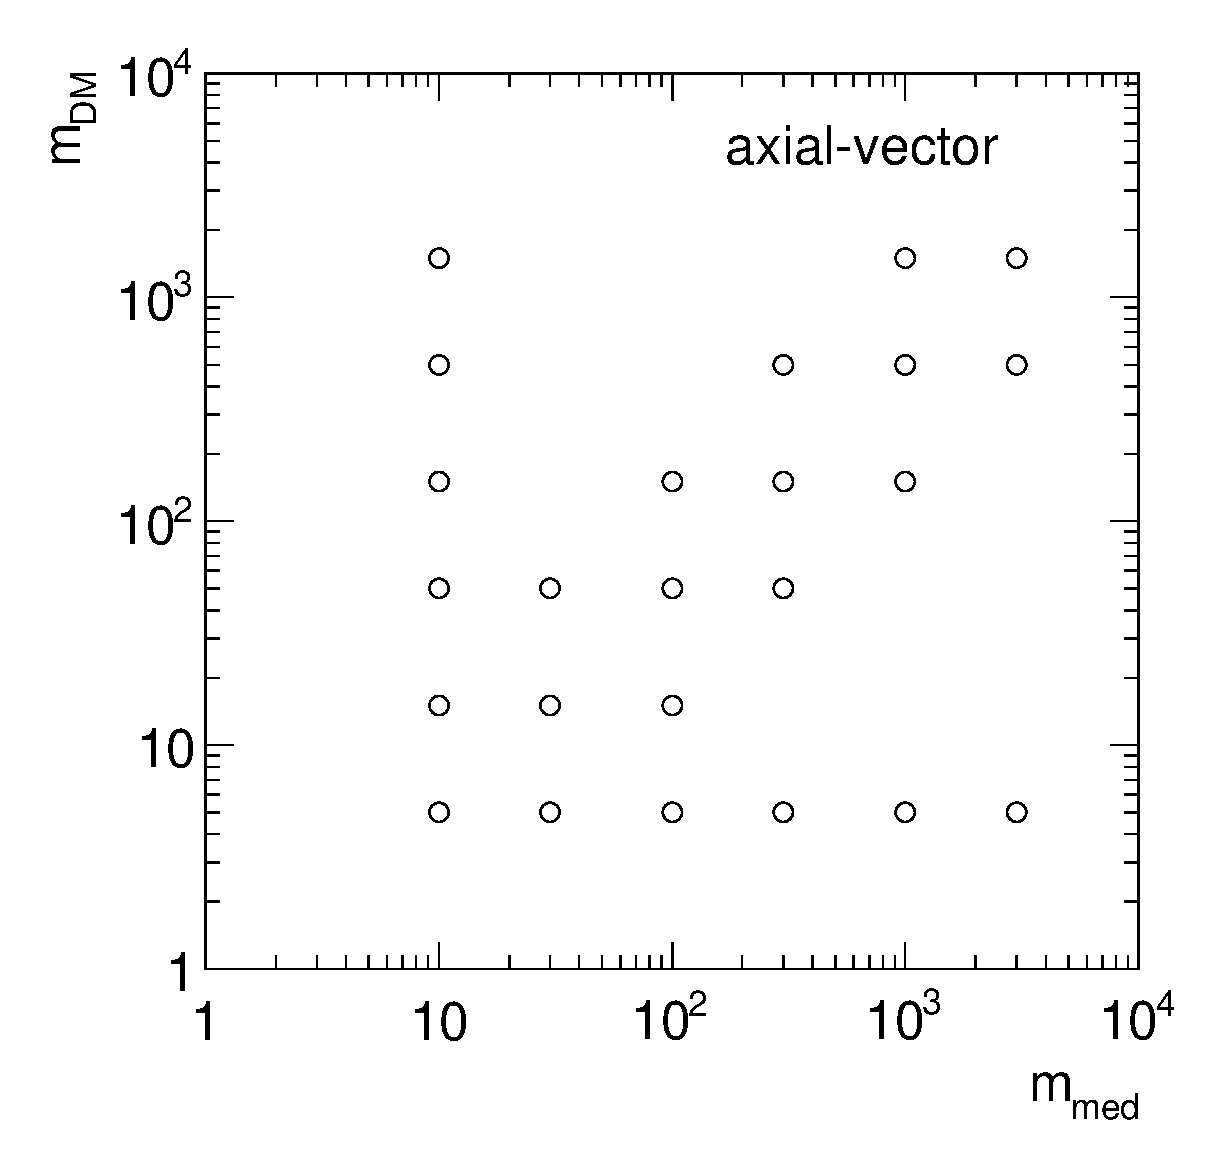
\includegraphics[width=0.45\linewidth]{figures/monojet/grid_A.eps}
\caption{Proposed parameter grid for vector and axial-vector mediator in the $\mMed$--$\mDM$ plane.}
\label{fig:monojet_grid_V}
\end{figure}

The presentation of the results in the $g_q$--$\gDM$ plane for fixed masses benefits from cross section scaling and is discussed in Section\,\ref{sec:monojet_scaling}.






\subsection{Scalar and pseudoscalar mediator, s-channel exchange}

%TODO add figure with diagrams

The matrix element implementation of the s-channel spin-0 mediated DM production is available in POWHEG with the full top-loop calculation at LO\,\cite{Haisch:2015ioa}.
The model assumes Dirac Dark Matter particles and is based on the minimal flavor violation (MFV), which motivates Higgs-like Yukawa couplings of the mediator to the Standard Model quarks. No other couplings, such as to leptons, are allowed in this model.
The following two cases are considered:\\
(a) scalar couplings to DM and SM,\\
(b) pseudo-scalar couplings to DM and SM\\
\noindent with the corresponding Lagrangians written as:
\begin{align}
\label{eq:SP} 
\mathcal{L}_{\mathrm{scalar}} &= g_q \sum \frac{m_q}{v} (\bar{q}q) S + \gDM (\bar{\chi}\chi) S \\
\mathcal{L}_{\mathrm{pseudo-scalar}} &= g_q \sum \frac{m_q}{v} (\bar{q}\gamma^5q) P + \gDM (\bar{\chi}\gamma^5\chi) P \\
\end{align}
where $v=246$\,GeV denotes the Higgs vacuum expectation value.

We choose to consider minimal mediator width given by Eq.\,\ref{eq:monojet_min}, where the individual contributions follow from
\begin{align}
\Gamma_{\bar{\chi}\chi}^{\rm{S}}&=\frac{\gDM^2 \mMed}{8\pi}\left(1-\frac{4 \mDM^2}{\mMed^2} \right)^{3/2}\\
\Gamma_{\bar{q}q}^{\rm{S}}&= \frac{3 \gq^2 \mMed}{8\pi}\frac{m_q^2}{v^2}\left(1-\frac{4 m_q^2}{\mMed^2}\right)^{3/2}\\
\Gamma_{\bar{\chi}\chi}^{\rm{P}}&=\frac{\gDM^2 \mMed}{8\pi} \sqrt{1-\frac{4 \mDM^2}{\mMed^2}}\\
\Gamma_{\bar{q}q}^{\rm{P}}&= \frac{3 \gq^2 \mMed}{8\pi}\frac{m_q^2}{v^2}\sqrt{1-\frac{4 m_q^2}{\mMed^2}}\label{eq:Gamma4}\;.
\end{align}
The minimal width for scalar and pseudo-scalar mediators with $g_q=\gDM=1$ are shown in Fig.\,\ref{fig:monojet_width_S}, illustrating the effect of the Higgs-like Yukawa couplings. For the mediator masses above twice the top quark mass $m_t$, the minimal width receives the dominant contribution from the top quark. For lighter mediator masses, Dark Matter dominates as the couplings to lighter quarks are Yukawa suppressed.
Note that we decide to ignore the partial width coming from gluons through loops as it can be safely neglected\,\cite{Haisch:2015ioa}.


\begin{figure}
\centering
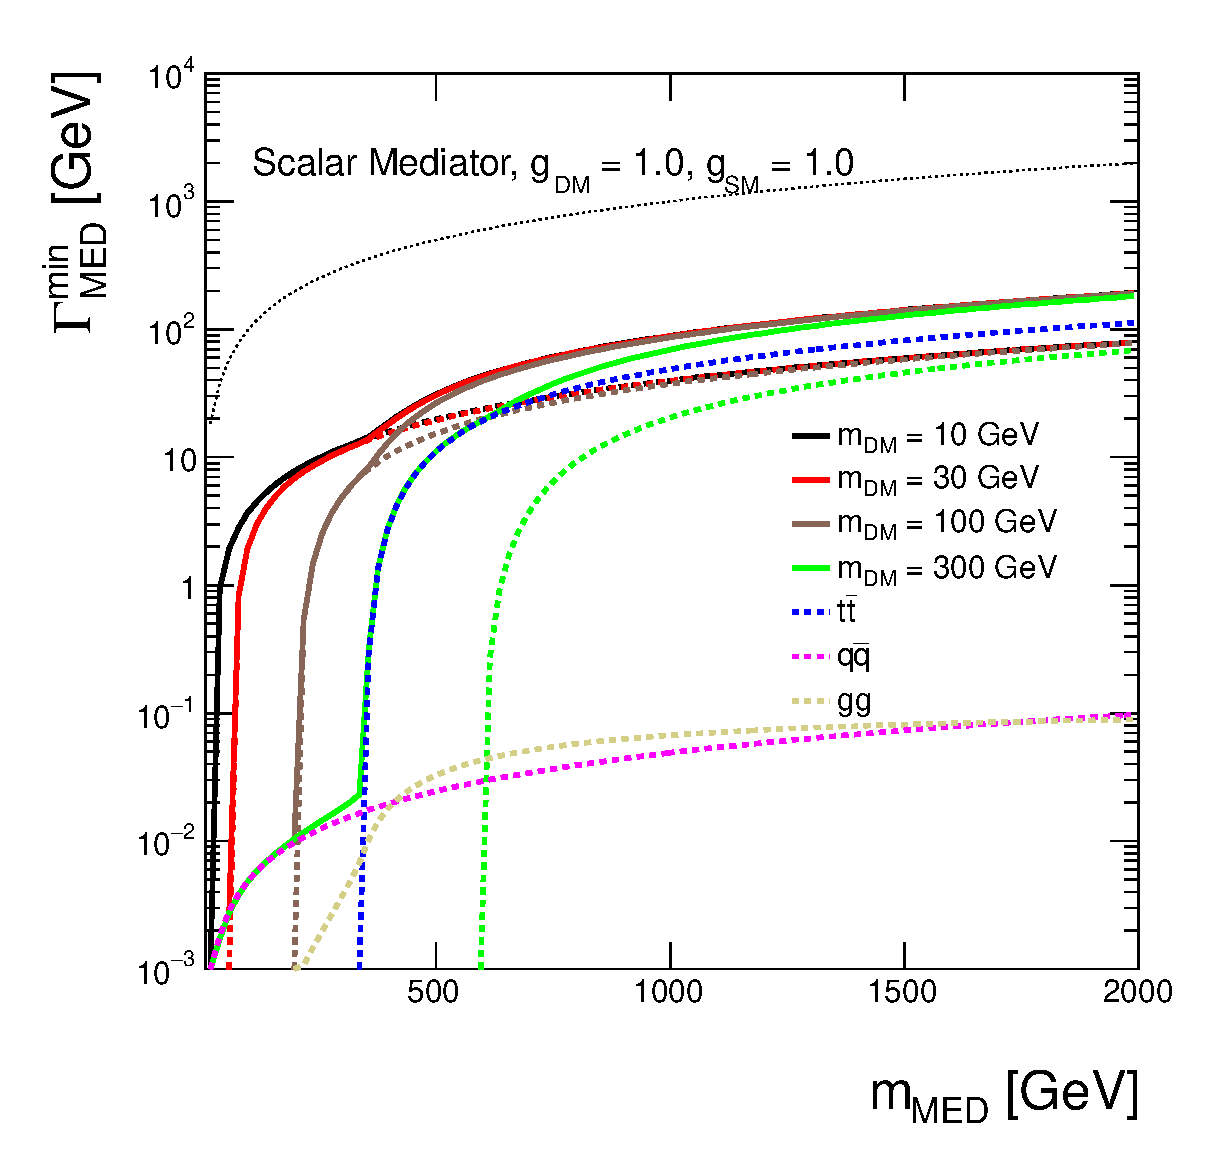
\includegraphics[width=0.45\linewidth]{figures/monojet/width_S.eps}
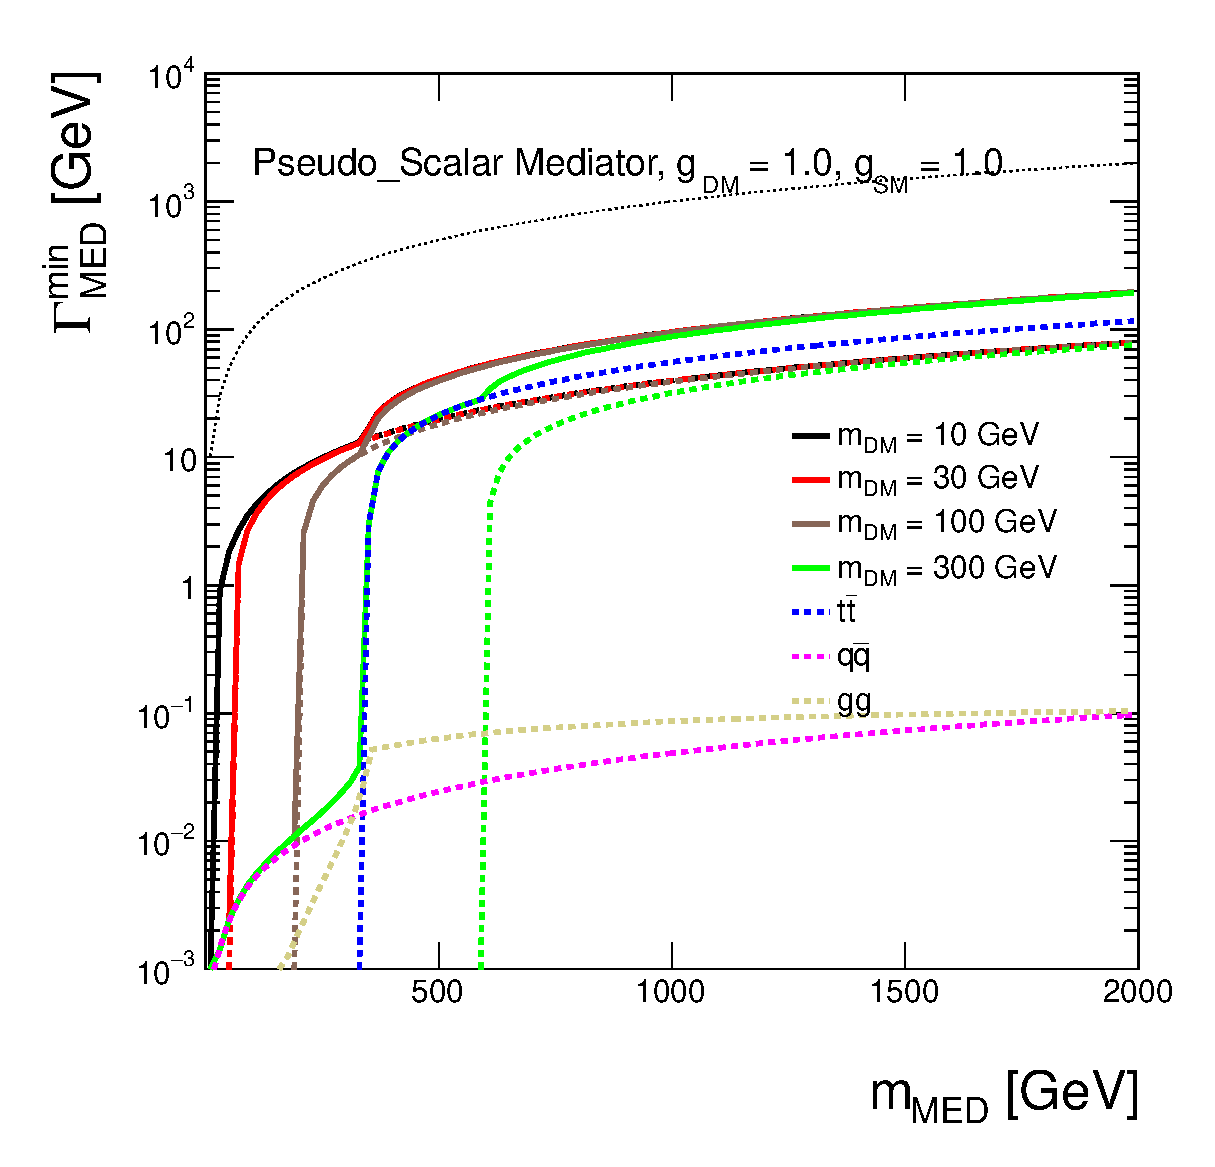
\includegraphics[width=0.45\linewidth]{figures/monojet/width_P.eps}
\caption{Minimal width as a function of mediator mass for scalar and pseudo-scalar mediator assuming couplings of 1. The total width is shown as solid lines for Dark Matter masses of 10\,GeV, 30\,GeV, 100\,GeV and 300\,GeV in black, red, brown and green, respectively. The individual contributions from Dark Matter are indicated by dotted lines with the same colors. The contribution from all quarks but top is shown as magenta dotted line and the contribution from top quarks only is illustrated by the dotted blue line. The dotted black line shows the extreme case $\Gamma_{\rm{min}}=\mMed$.}
\label{fig:monojet_width_S}
\end{figure}


Similarly as in the case of the vector and axial-vector mediators, scans in the paramater space are performed also for the scalar and pseudo-scalar mediators in order to decide on the optimised parameter grid for the presentation of Run-2 results. Figures\,\ref{fig:monojet_scan_S_g,fig:monojet_scan_S_mDM1000,fig:monojet_scan_S_mDM100,fig:monojet_scan_S_mMed10,fig:monojet_scan_S_mMed1000} show the scans over the couplings, Dark Matter mass and mediator mass and the same conclusions apply as in Section\,\ref{sec:monojet_V}.

%TODO does the discussion below make sense?
Since the top quark gives the dominant contribution to the mediator width due to Higgs-like Yukawa couplings, the effect of the top channel opening in the mediator production was studied in addition. Scan over the mediator mass is shown in Fig.\,\ref{fig:monojet_scan_S_mMed1000} where the mediator masses 300\,GeV and 500\,GeV are chosen to be below and above $2m_t$. The off-shell Dark Matter production regime is assumed by taking $\mDM=1$\,TeV in order to allow studying solely the effects of the couplings to quarks. 
No differences in the kinematic distributions are observed and also the cross sections remain similar in this case. Therefore, it is concluded that no significant changes appear for mediator masses around the $2m_t$ threshold.

\begin{figure}
\centering
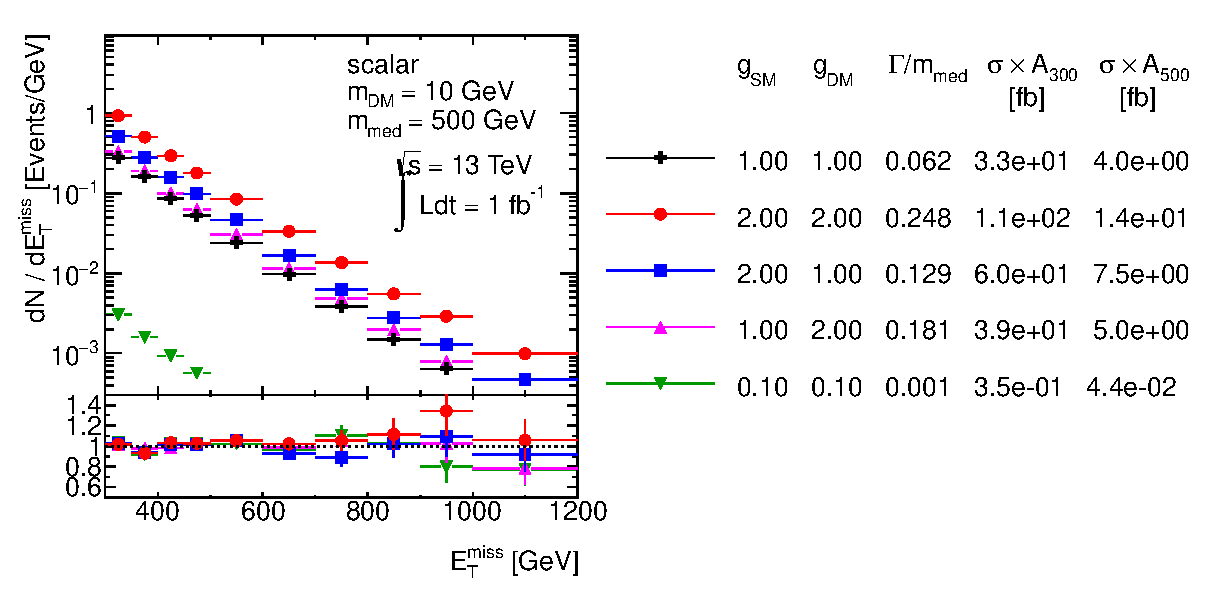
\includegraphics[width=0.9\linewidth]{figures/monojet/scan_g_S_10_500.eps}
\caption{Scan over couplings. The $\MET$ distribution is compared for the scalar mediator models using the parameters as indicated. Ratios of the normalized distributions with respect to the first one are shown. $A_{300}$ and $A_{500}$ in the table denote the acceptance of the $\MET>300$\,GeV and $\MET>500$\,GeV cut, respectively.}
\label{fig:monojet_scan_S_g}
\end{figure}

\begin{figure}
\centering
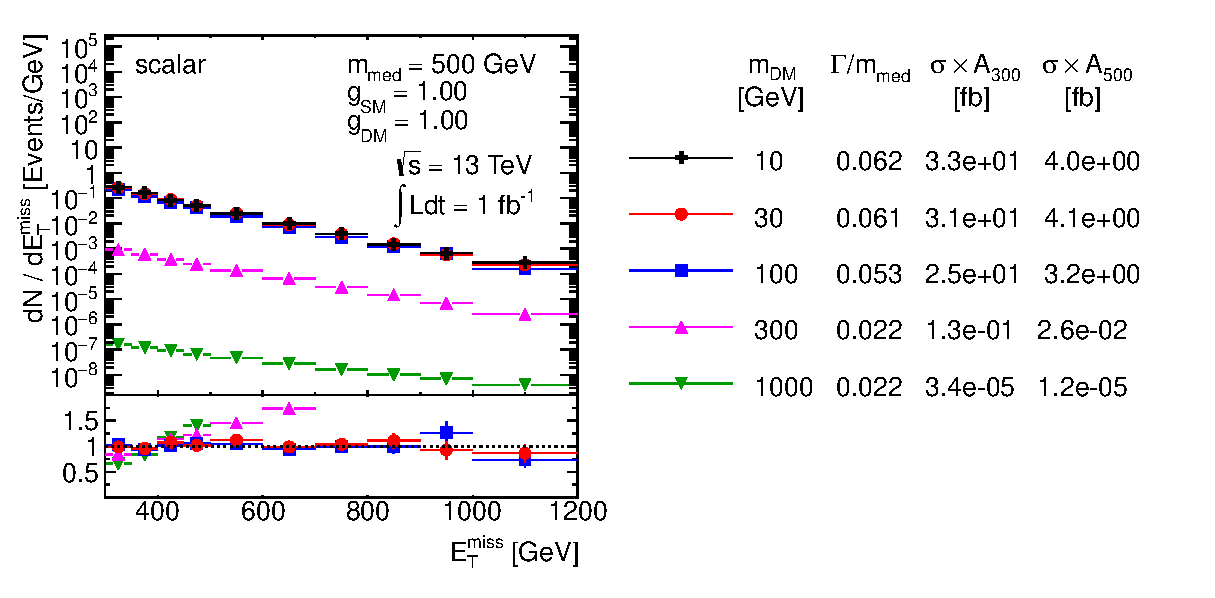
\includegraphics[width=0.9\linewidth]{figures/monojet/scan_mDM_S_500.eps}
\caption{Scan over Dark Matter mass. The $\MET$ distribution is compared for the scalar mediator models using the parameters as indicated. Ratios of the normalized distributions with respect to the first one are shown. $A_{300}$ and $A_{500}$ in the table denote the acceptance of the $\MET>300$\,GeV and $\MET>500$\,GeV cut, respectively.}
\label{fig:monojet_scan_S_mDM1000}
\end{figure}

\begin{figure}
\centering
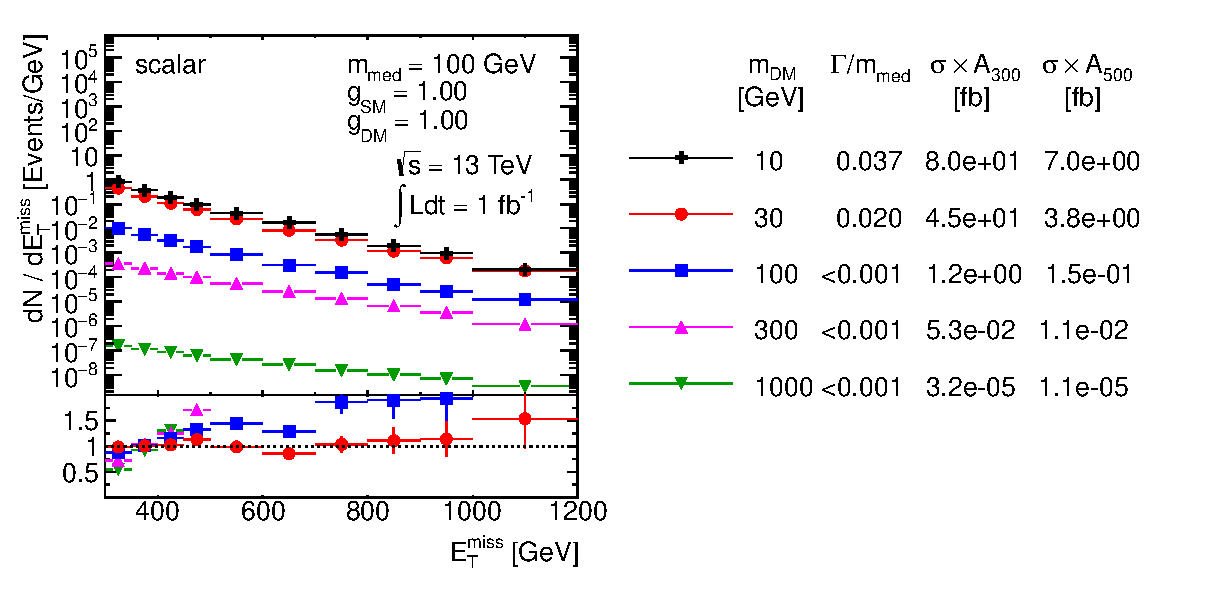
\includegraphics[width=0.9\linewidth]{figures/monojet/scan_mDM_S_100.eps}
\caption{Scan over Dark Matter mass. The $\MET$ distribution is compared for the scalar mediator models using the parameters as indicated. Ratios of the normalized distributions with respect to the first one are shown. $A_{300}$ and $A_{500}$ in the table denote the acceptance of the $\MET>300$\,GeV and $\MET>500$\,GeV cut, respectively.}
\label{fig:monojet_scan_S_mDM100}
\end{figure}

\begin{figure}
\centering
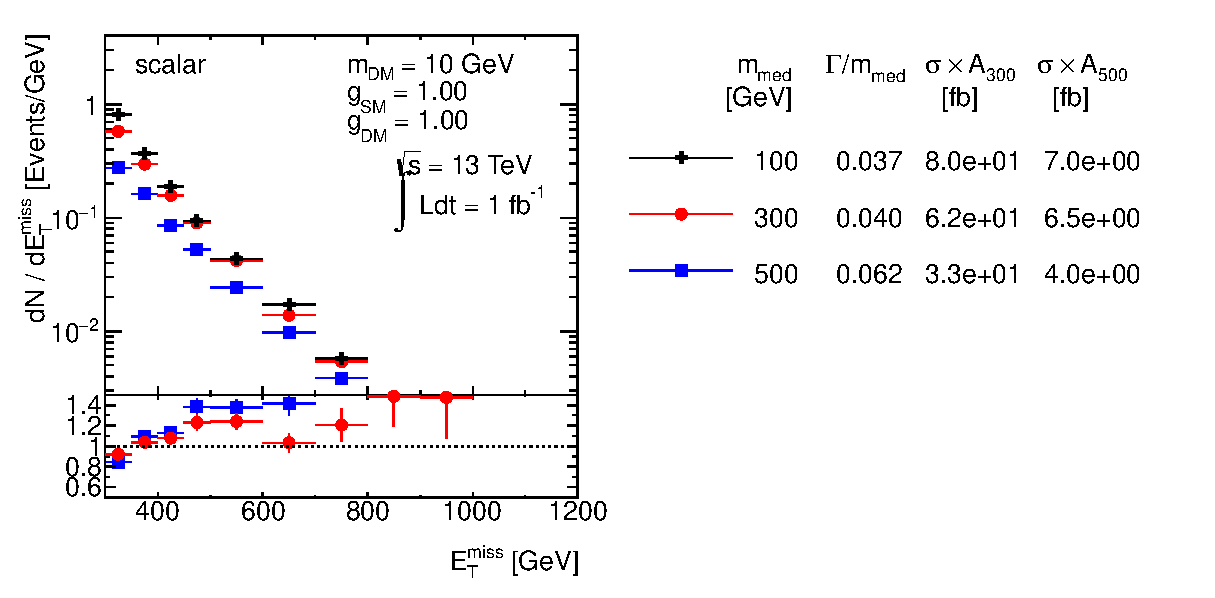
\includegraphics[width=0.9\linewidth]{figures/monojet/scan_mMed_S_10.eps}
\caption{Scan over mediator mass. The $\MET$ distribution is compared for the scalar mediator models using the parameters as indicated. Ratios of the normalized distributions with respect to the first one are shown. $A_{300}$ and $A_{500}$ in the table denote the acceptance of the $\MET>300$\,GeV and $\MET>500$\,GeV cut, respectively.}
\label{fig:monojet_scan_S_mMed10}
\end{figure}

\begin{figure}
\centering
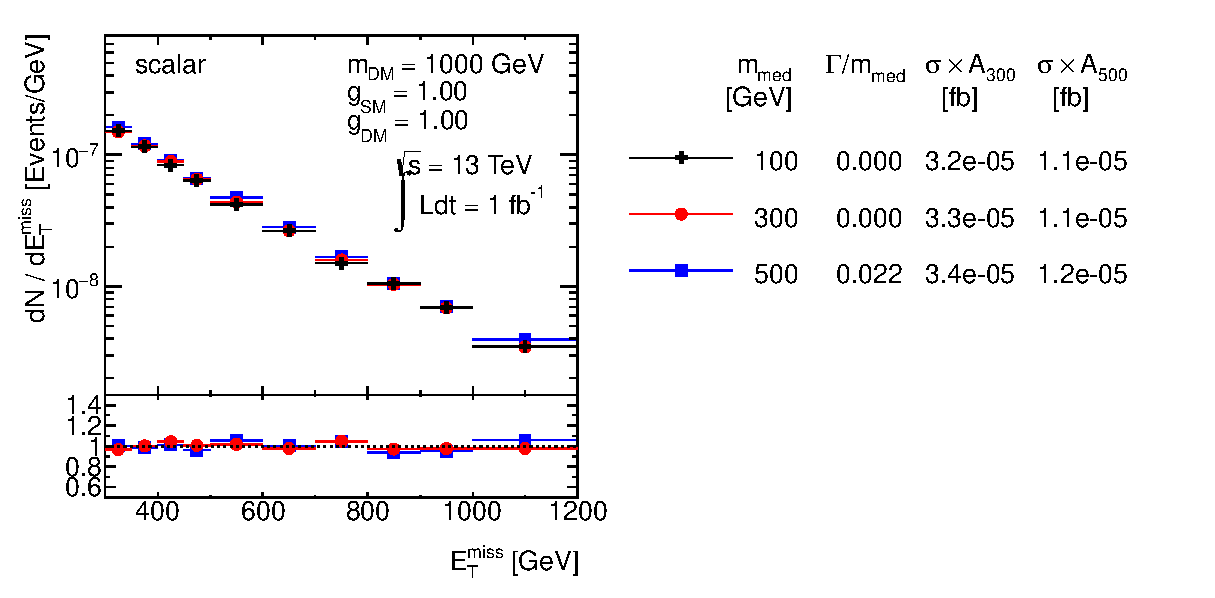
\includegraphics[width=0.9\linewidth]{figures/monojet/scan_mMed_S_1000.eps}
\caption{Scan over mediator mass. The $\MET$ distribution is compared for the scalar mediator models using the parameters as indicated. Ratios of the normalized distributions with respect to the first one are shown. $A_{300}$ and $A_{500}$ in the table denote the acceptance of the $\MET>300$\,GeV and $\MET>500$\,GeV cut, respectively.}
\label{fig:monojet_scan_S_mMed1000}
\end{figure}


The optimized parameter grid in the $\mMed$--$\mDM$ plane for scalar and pseudo-scalar mediators is motivated by similar arguments as in the previous section. Therefore, similar pattern is followed here, taking again $g_q=\gDM=1$. Only the sensitivity to the highest mediator masses has to be revisited.
The generator level cross section times the acceptance at $\MET>500$\,GeV for the model with couplings $g_q=\gDM=1$, light Dark Matter of 10\,GeV and 500\,GeV scalar mediator is at the order of 10\,fb, i.e. just at the edge of the early Run-2 sensitivity. Increasing the mediator mass to 1\,TeV pushes the product $\sigma\times A$ down to approximately 0.1\,fb, beyond the LHC sensitivity. Therefore, we choose to remove the 3\,TeV mediator mass from the grid and present the final grid with 19 mass points only in Fig.\,\ref{fig:monojet_grid_S}.
%mDM =    5  : mMed =   10    30   100   300  1000 
%mDM =   15  : mMed =   10    30   100              
%mDM =   50  : mMed =   10    30   100   300        
%mDM =  150  : mMed =   10         100   300  1000  
%mDM =  500  : mMed =   10               300  1000

\begin{figure}
\centering
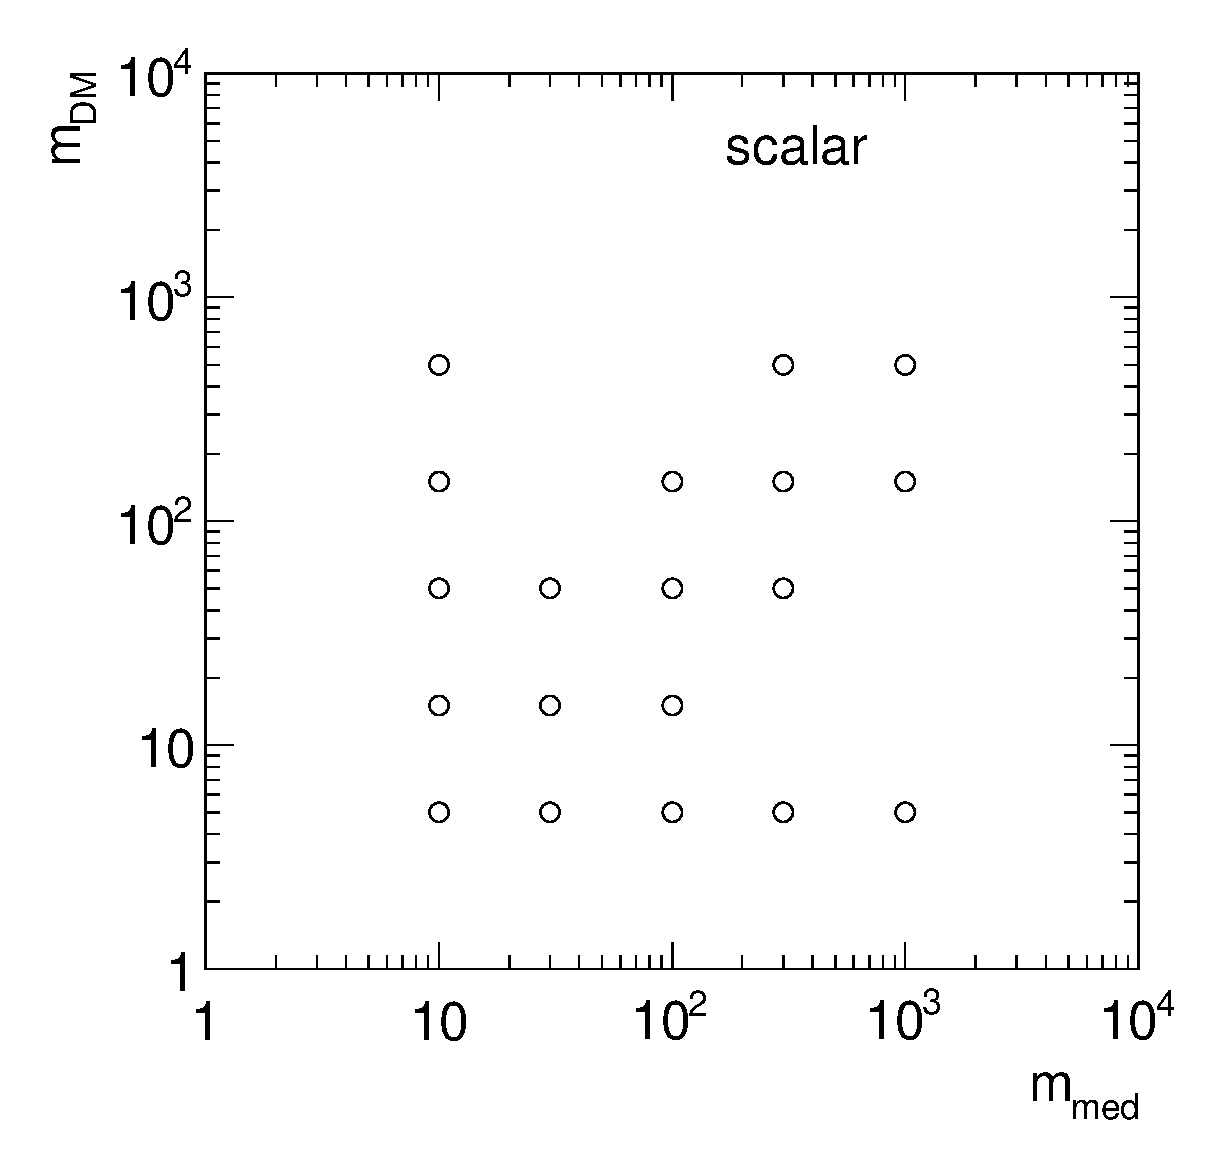
\includegraphics[width=0.45\linewidth]{figures/monojet/grid_S.eps}
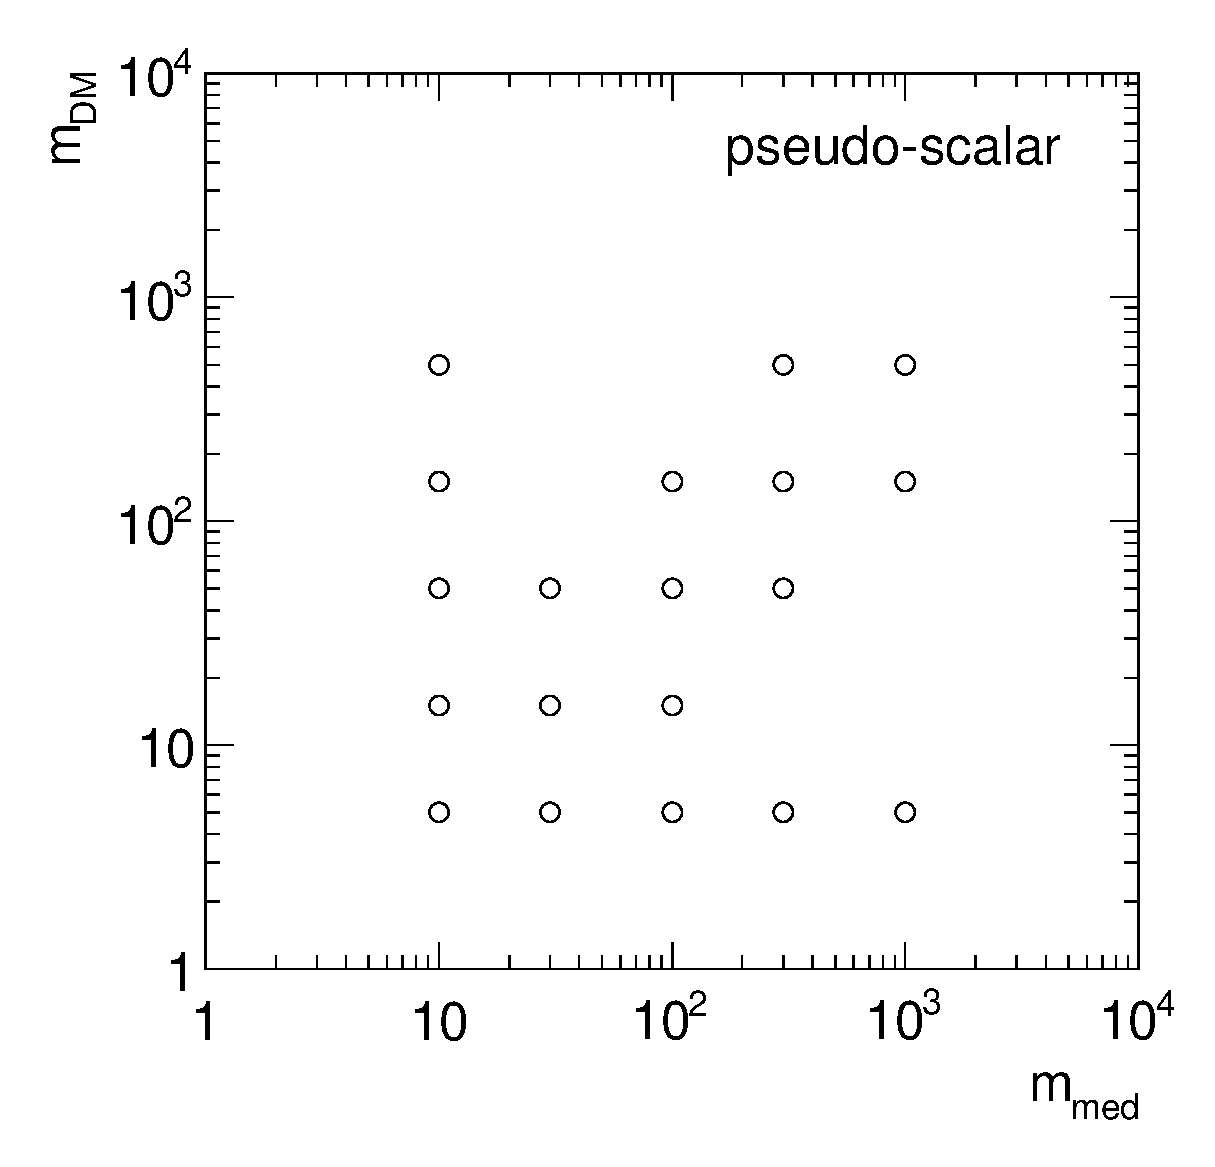
\includegraphics[width=0.45\linewidth]{figures/monojet/grid_P.eps}
\caption{Proposed parameter grid for scalar and pseudo-scalar mediator in the $\mMed$--$\mDM$ plane.}
\label{fig:monojet_grid_S}
\end{figure}

The proposal for the scan in the $g_q$--$\gDM$ plane is described in the following section.






\subsection{Cross section scaling}
\label{sec:monojet_scaling}

The aim of the parameter grid optimization is to find out whether certain parts of the parameter space can be omitted and one can rely on the neighboring grid points in order to populate the missing parts. There are two ways of doing this:
\begin{itemize}
\item Interpolation is used in-between the grid points that are close enough such that finer granularity is not needed for the presentation purposes, or between the points where smooth or no changes of the results are expected. The latter argument is exactly the one that motivates the reduction of the grid points in the $\mMed$--$\mDM$ plane.\\
\item Recalculation of the results can be used when the dependencies with respect to the neighboring grid points are known.\\
\end{itemize}

The results of the scan over the couplings presented in the previous sections indicate there are no changes in kinematic distributions for different choices of the coupling strengths. This means that the acceptance remains the same in the whole $g_q$--$\gDM$ plane and it is sufficient to perform the detector simulation only for one single grid point. The resulting truth-level selection acceptance and the detector reconstruction efficiency can then be applied to all remaining grid points in the $g_q$--$\gDM$ plane where only the generator-level cross section needs to be known. This significantly reduces the computing time as the detector response is by far the most expensive part of the Monte Carlo sample production. However, a further step can be taken if a parameterization of the cross section dependence from one grid point to another exists, in which case the number of generated samples can be reduced even further.

Let us now elaborate on a cross section scaling procedure.
%TODO say something about the fact that this can work only for fixed masses
The propagator on the s-channel exchange is written in a Breit-Wigner form as $\frac{1}{\sqrt{s}-\mMed^2 + i\mMed\Gamma}$. The relative size of the center-of-mass energy defined by the two partons entering the hard process and the mediator mass allows to classify the production in the following way:
\begin{itemize}
\item off-shell production when $\sqrt{s} \gg \mMed$ leading to suppressed cross sections,
\item on-shell production when $\sqrt{s} \sim \mMed$ leading to enhanced cross sections,
\item effective field theory (EFT) limit when $\sqrt{s} \ll \mMed$.
\end{itemize}
All three categories can be distinguished in Fig.\,\ref{fig:monojet_MstarMmed} showing the upper limit on the interaction scale $M^{*} \equiv \mMed/\sqrt{g_q\gDM}$ for vector mediator. 
In the case of the off-shell production and the EFT limit, the first term in the propagator dominates which reduces the dependence on the mediator width. Therefore, in these cases one can approximate the cross section as
\begin{equation}
\sigma \propto g_q^2\gDM^2.
\end{equation}
The on-shell production regime is the most interesting one as it gives the best chances for a discovery at the LHC given the cross section enhancement. The propagator term with the width cannot be neglected in this case and, in the narrow width approximation, one can integrate
\begin{equation}
\int \frac{ds}{(s-\mMed^2)^2 + \mMed^2\Gamma^2} = \frac{\pi}{\mMed\Gamma}
\end{equation}
which further implies the cross section scaling
\begin{equation}
\sigma \propto \frac{g_q^2\gDM^2}{\Gamma}.
\label{eq:monojet_scaling}
\end{equation}
Since $\Gamma \sim g_q^2+\gDM^2$, one can simplify this rule in the extreme cases as follows
\begin{eqnarray}
\sigma &\propto& \frac{g_q^2\gDM^2}{g_q^2+\gDM^2} \xrightarrow{g_q \ll \gDM} g_q^2 \label{eq:monojet_gSM} \\
\sigma &\propto& \frac{g_q^2\gDM^2}{g_q^2+\gDM^2} \xrightarrow{g_q \gg \gDM} \gDM^2 \label{eq:monojet_gDM} \;.
\end{eqnarray}
However, it is important to keep in mind that there is no simple scaling rule for how the cross section changes with the Dark Matter mass, mediator mass and the mediator width because PDFs matter in such cases as well.
%The only case where there is a simple scaling with mass is if one mass is much smaller than the other mass, in which case the cross section becomes independent of the smaller mass.
Therefore, the scaling procedure outlined above is expected to work only for fixed masses and fixed mediator width.


\begin{figure}
\centering
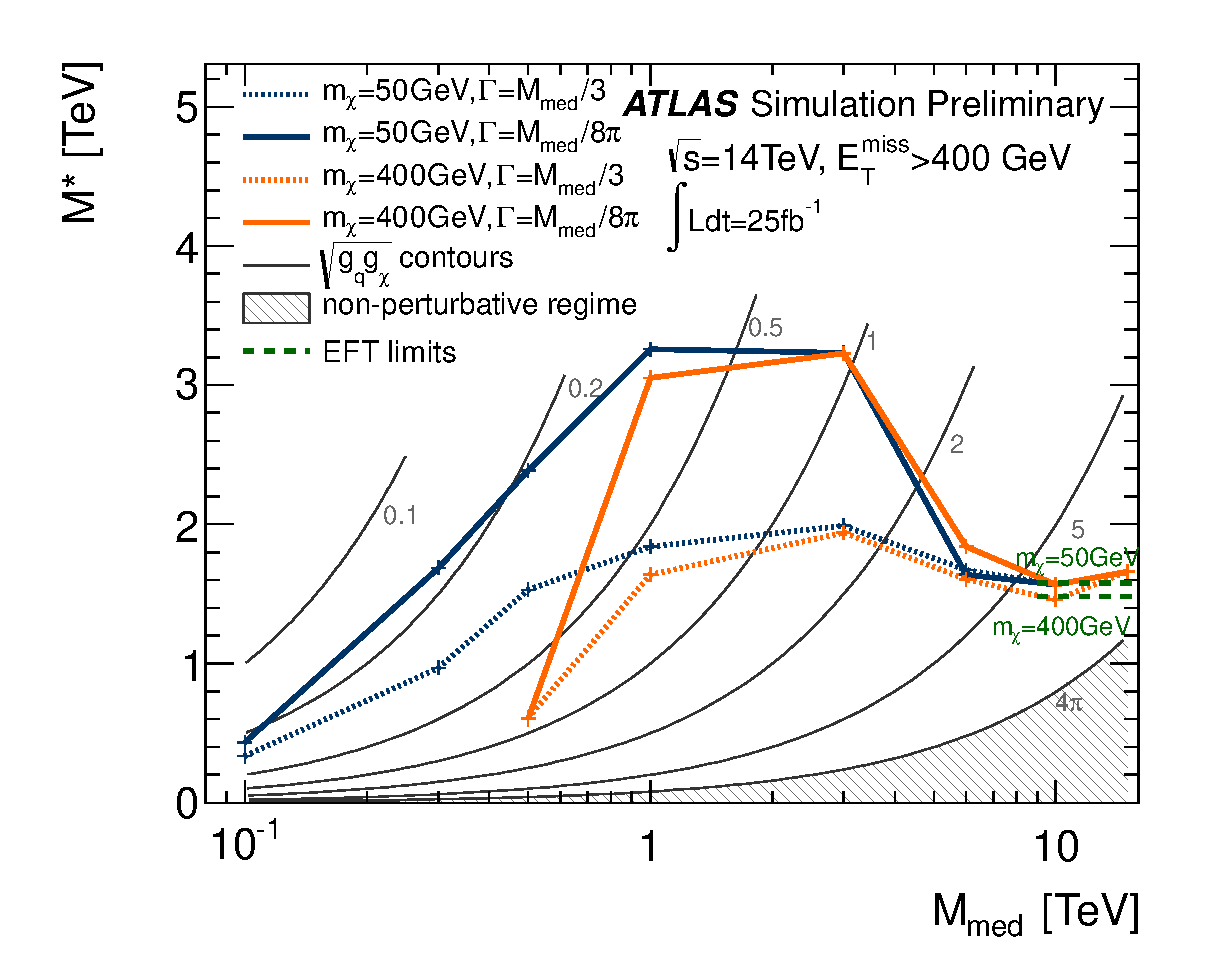
\includegraphics[width=0.9\linewidth]{figures/monojet/lambda_14TeV_SR1.eps}
\caption{Comparison of the 95\% CL lower limits on the scale of the interaction of a $Z'$-like simplified model at 14\,TeV, in terms of the mediator mass. Corresponding limits from EFT models are shown on the same plot as green dashed lines to show equivalence between the two models for high mediator masses.
Taken from Ref.\,\cite{ATL-PHYS-PUB-2014-007}.}
\label{fig:monojet_MstarMmed}
\end{figure}



Figures\,\ref{fig:monojet_width100} and \ref{fig:monojet_width1000} show the minimal width in the $g_q$--$\gDM$ plane for all vector, axial-vector, scalar and pseudo-scalar mediators for $\mMed=100$\,GeV and 1000\,GeV, respectively, taking $\mDM=10$\,GeV. The individual colors indicate the lines of constant width along which the cross section scaling works. For vector and axial-vector mediators, the minimal width is predominantly defined by $g_q$ due to the number of quark flavors and the color factor. %In this case, the scaling follows from Eq.\,\ref{eq:monojet_gDM}.
On the contrary, both the Standard Model and Dark Matter partial width have comparable contributions in case of scalar and pseudo-scalar mediators if the top quark channel is open ($\mMed>2m_t$). However, mostly $\gDM$ defines the minimal width for $\mMed<2m_t$ due to the Yukawa-suppressed light quark couplings.


\begin{figure}
\centering
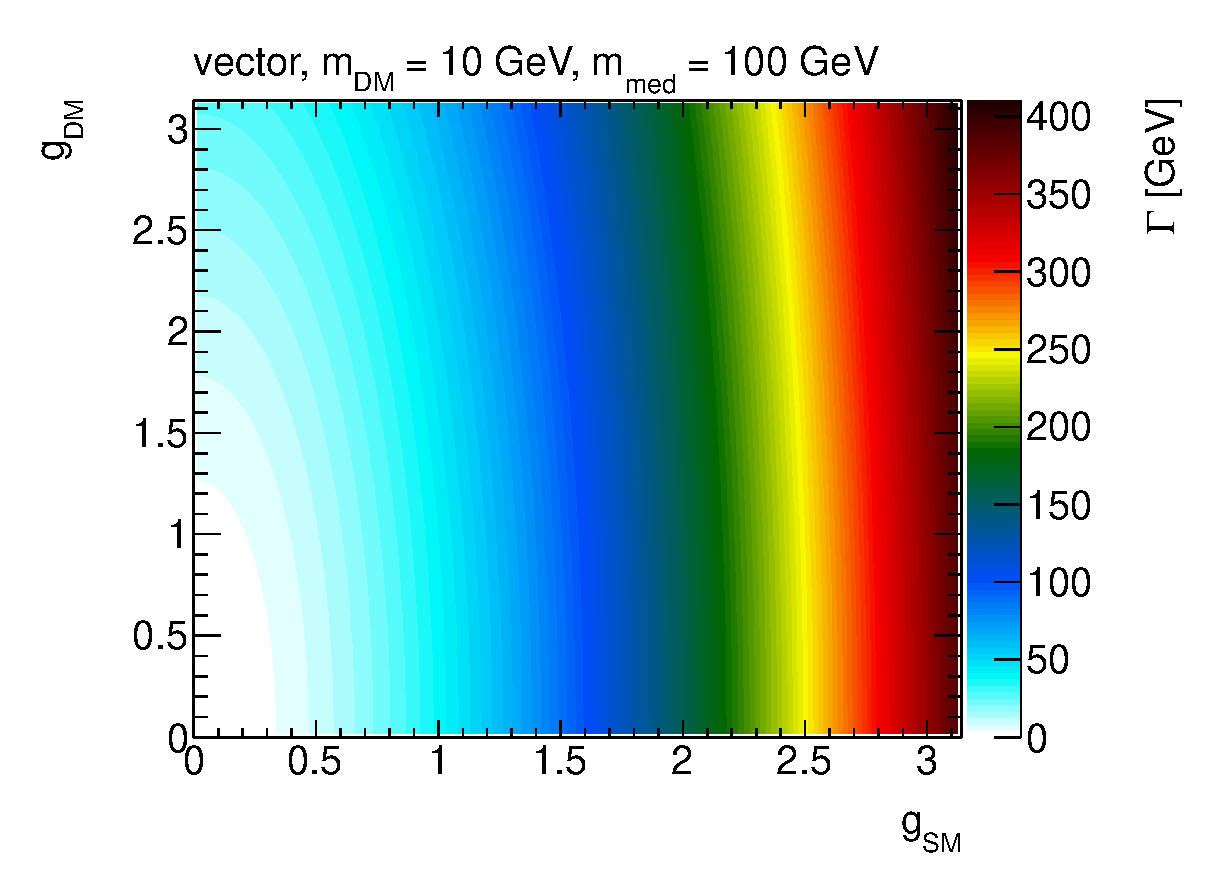
\includegraphics[width=0.45\linewidth]{figures/monojet/constantwidth_V_gg100.eps}
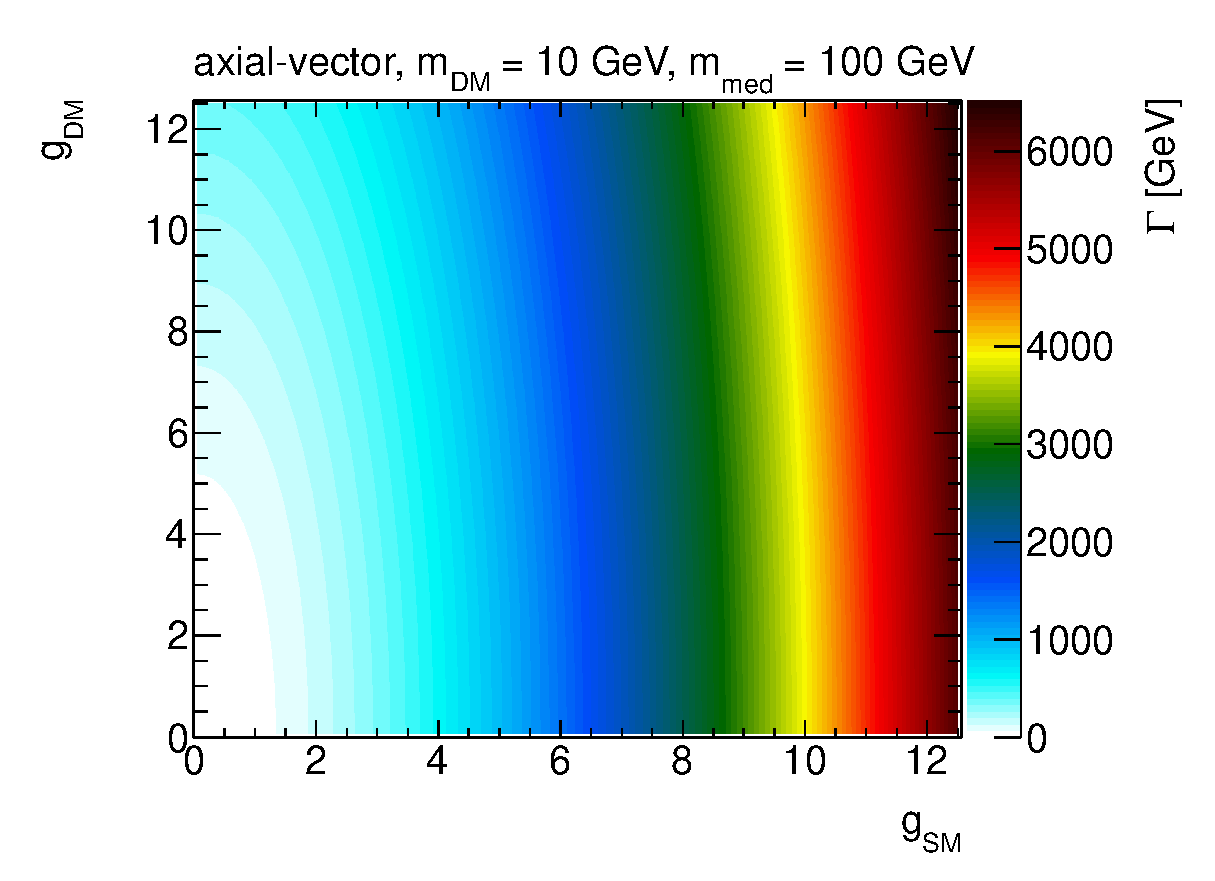
\includegraphics[width=0.45\linewidth]{figures/monojet/constantwidth_A_gg100.eps}\\
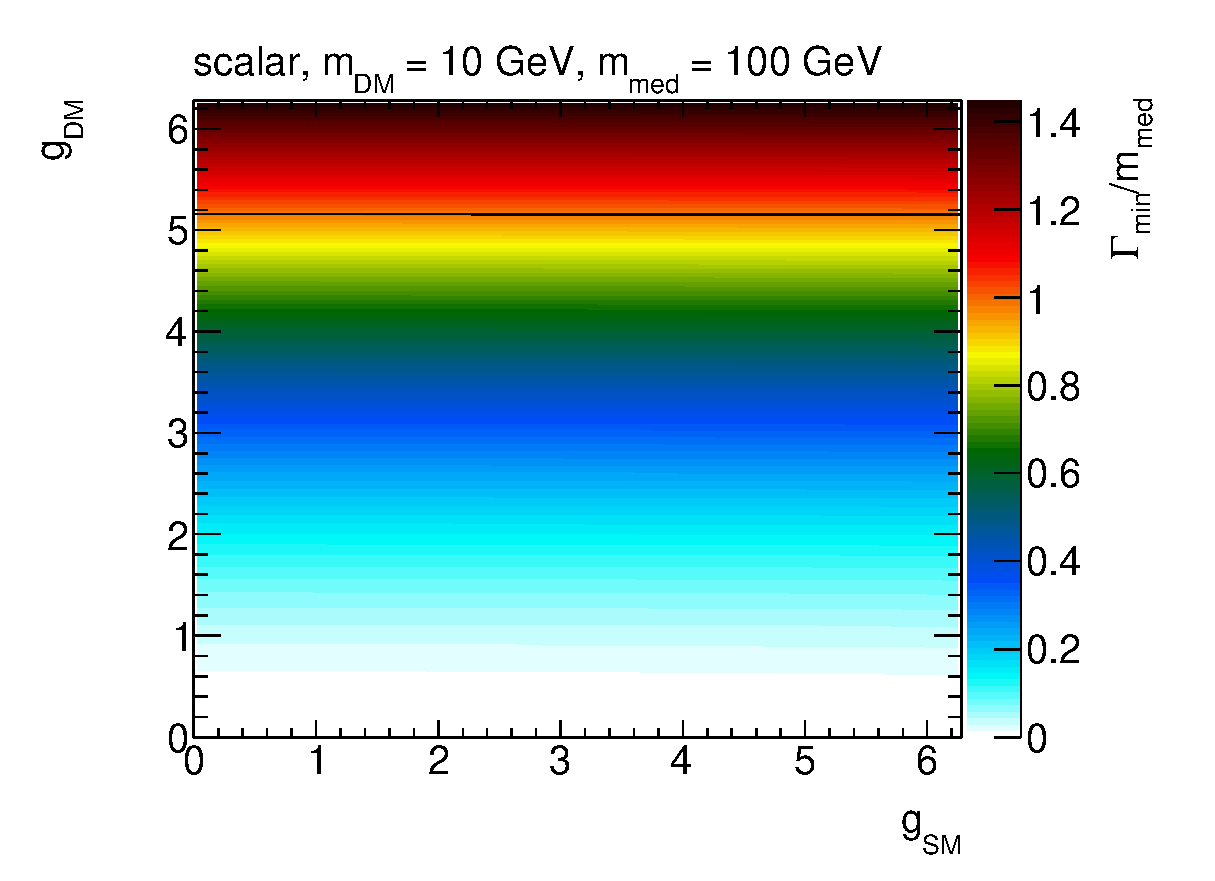
\includegraphics[width=0.45\linewidth]{figures/monojet/constantwidth_S_gg100.eps}
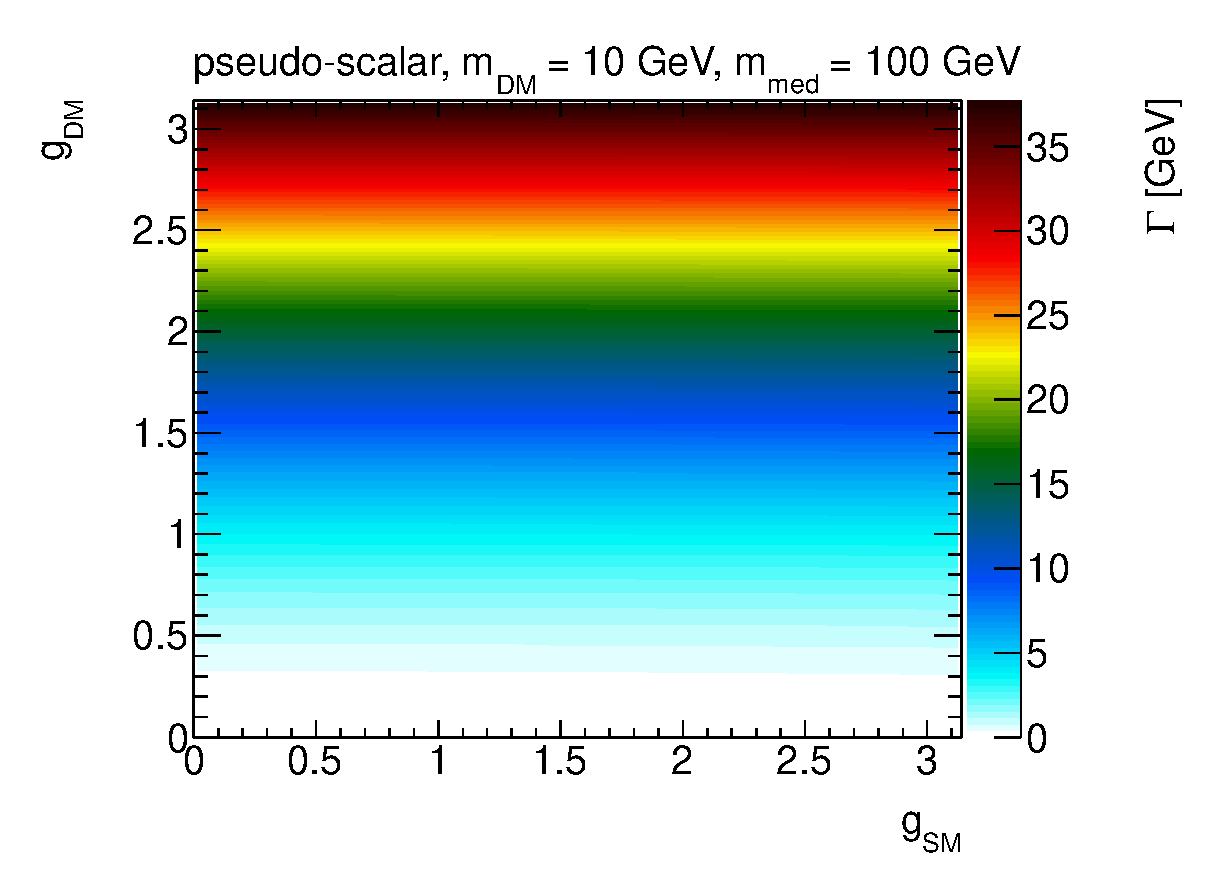
\includegraphics[width=0.45\linewidth]{figures/monojet/constantwidth_P_gg100.eps}
\caption{Minimal width for vector, axial-vector, scalar and pseudo-scalar mediators as a function of the individual couplings $g_q$ and $\gDM$, assuming $\mMed=100$\,GeV and $\mDM=10$\,GeV.}
%TODO indicate mMed=GammaMin in the plot (gDM = 6, gSM = 1.5 for V and gSM = gDM = 5 for S) 
\label{fig:monojet_width100}
\end{figure}

\begin{figure}
\centering
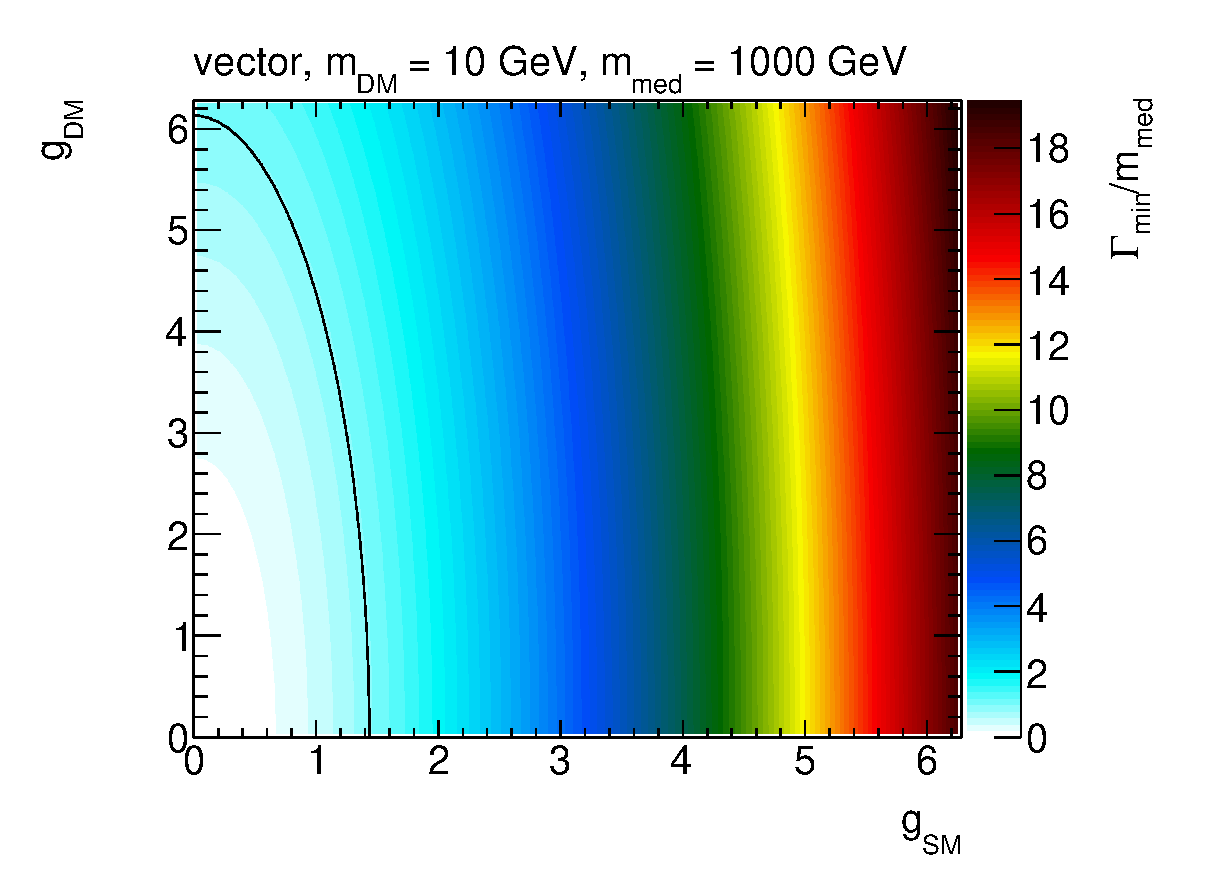
\includegraphics[width=0.45\linewidth]{figures/monojet/constantwidth_V_gg1000.eps}
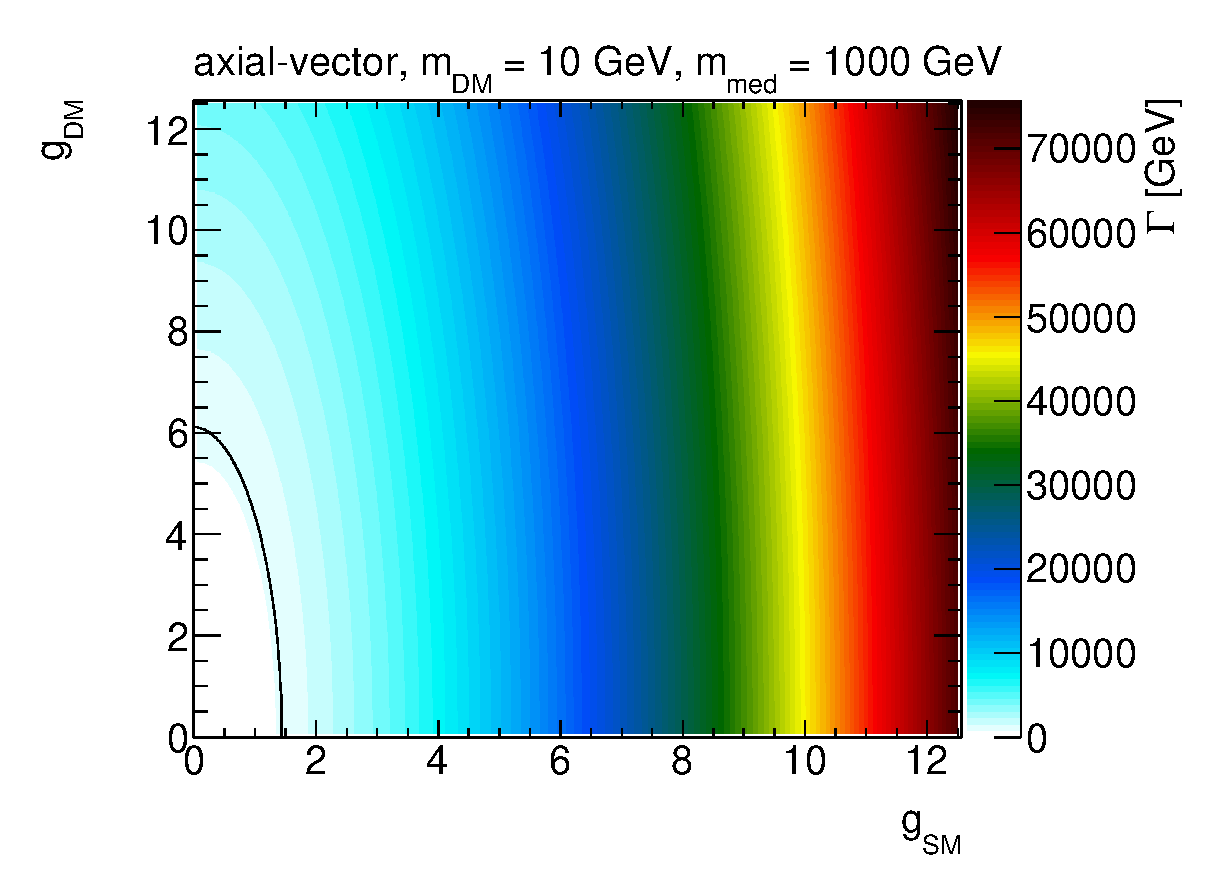
\includegraphics[width=0.45\linewidth]{figures/monojet/constantwidth_A_gg1000.eps}\\
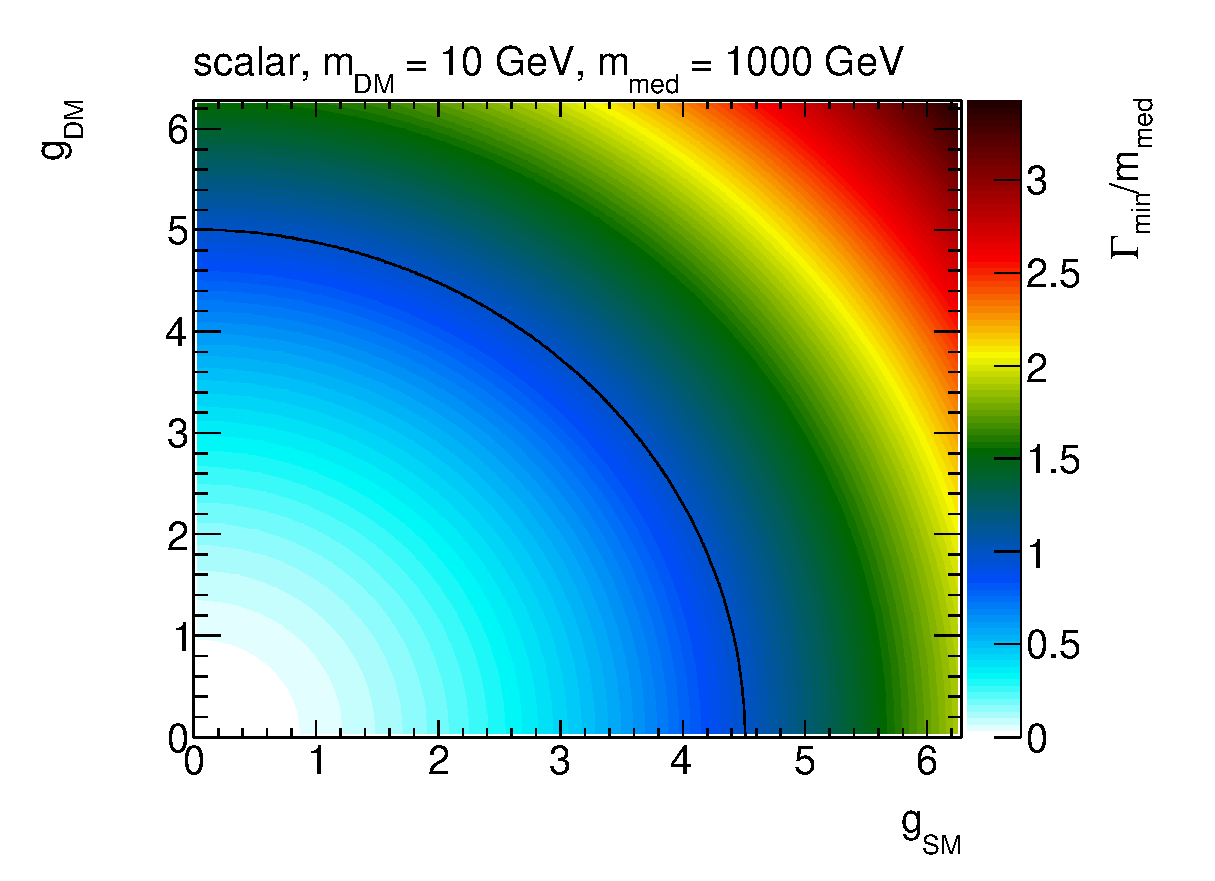
\includegraphics[width=0.45\linewidth]{figures/monojet/constantwidth_S_gg1000.eps}
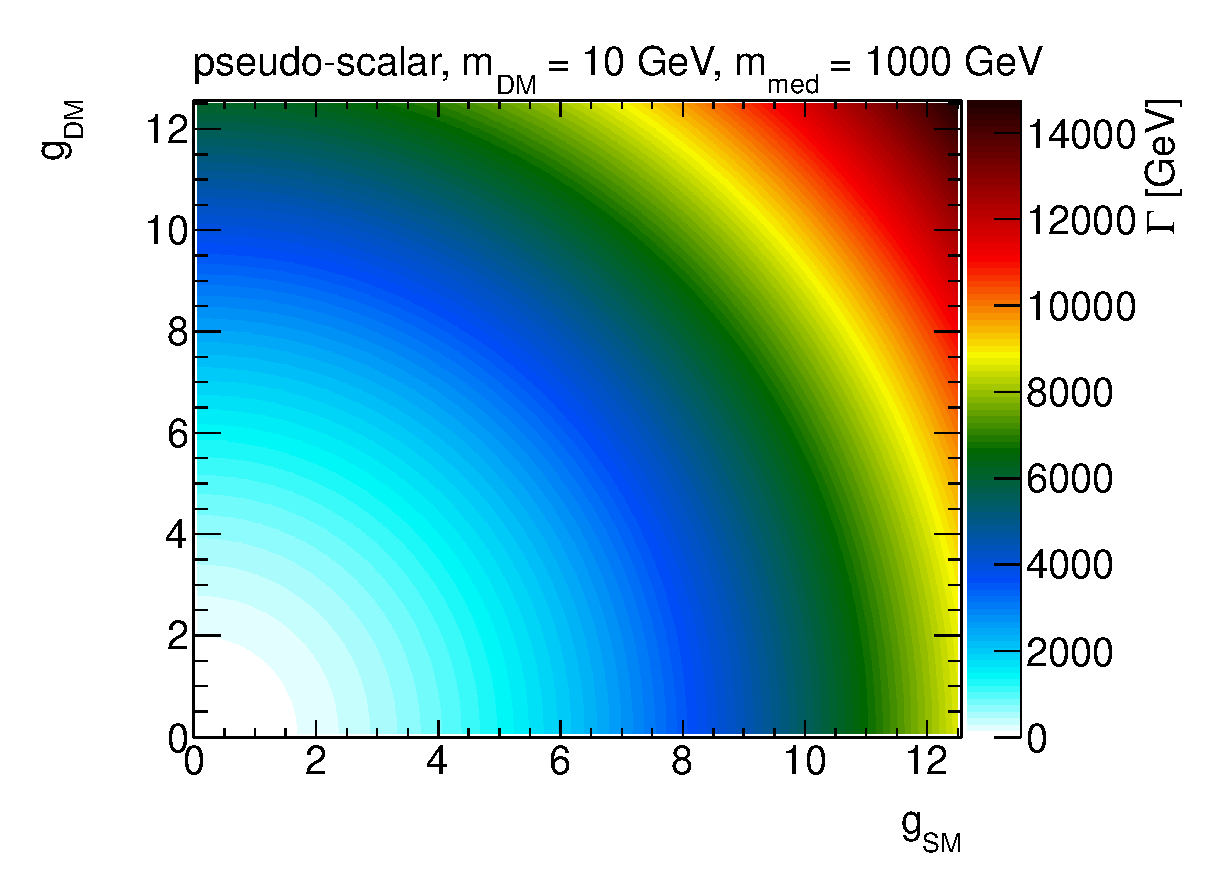
\includegraphics[width=0.45\linewidth]{figures/monojet/constantwidth_P_gg1000.eps}
\caption{Minimal width for vector, axial-vector, scalar and pseudo-scalar mediators as a function of the individual couplings $g_q$ and $\gDM$, assuming $\mMed=1$\,TeV and $\mDM=10$\,GeV.}
%TODO indicate mMed=GammaMin in the plot (gDM = 6, gSM = 1.5 for V and gSM = gDM = 5 for S) 
\label{fig:monojet_width1000}
\end{figure}


The performance of the cross section scaling is demonstrated in Fig.\,\ref{fig:monojet_scaling} %where two mass points $\mMed=100$\,GeV and 1\,TeV are chosen with $\mDM=10$\,GeV
where the mass point $\mMed=1$\,TeV and $\mDM=10$\,GeV is chosen
and rescaled from the starting point $g_q=\gDM=1$ according to Eq.\,\ref{eq:monojet_scaling} to populate the whole $g_q$--$\gDM$ plane. This means the width is not kept constant in this test and this is done in purpose in order to point out deviations from the scaling when the width is altered. For each mass point, the rescaled cross section is compared to the generator cross section and the ratio of the two is plotted.
For the given choice of the mass points, the scaling seems to work approximately with the precision of $\sim20\%$ in the region where $\Gamma_{\rm{min}}<\mMed$.
Constant colors indicate the lines along which the cross section scaling works precisely and there is a remarkable resemblance of the patterns shown in the plots of the mediator width. To prove the scaling along the lines of constant width works, one such line is chosen in Fig.\,\ref{fig:monojet_scaling_constwidth} for a scalar mediator, defined by $\mMed=300$\,GeV, $\mDM=100$\,GeV, $g_q=\gDM=1$, and the rescaled and generated cross sections are found to agree within 3\%.


\begin{figure}
\centering
%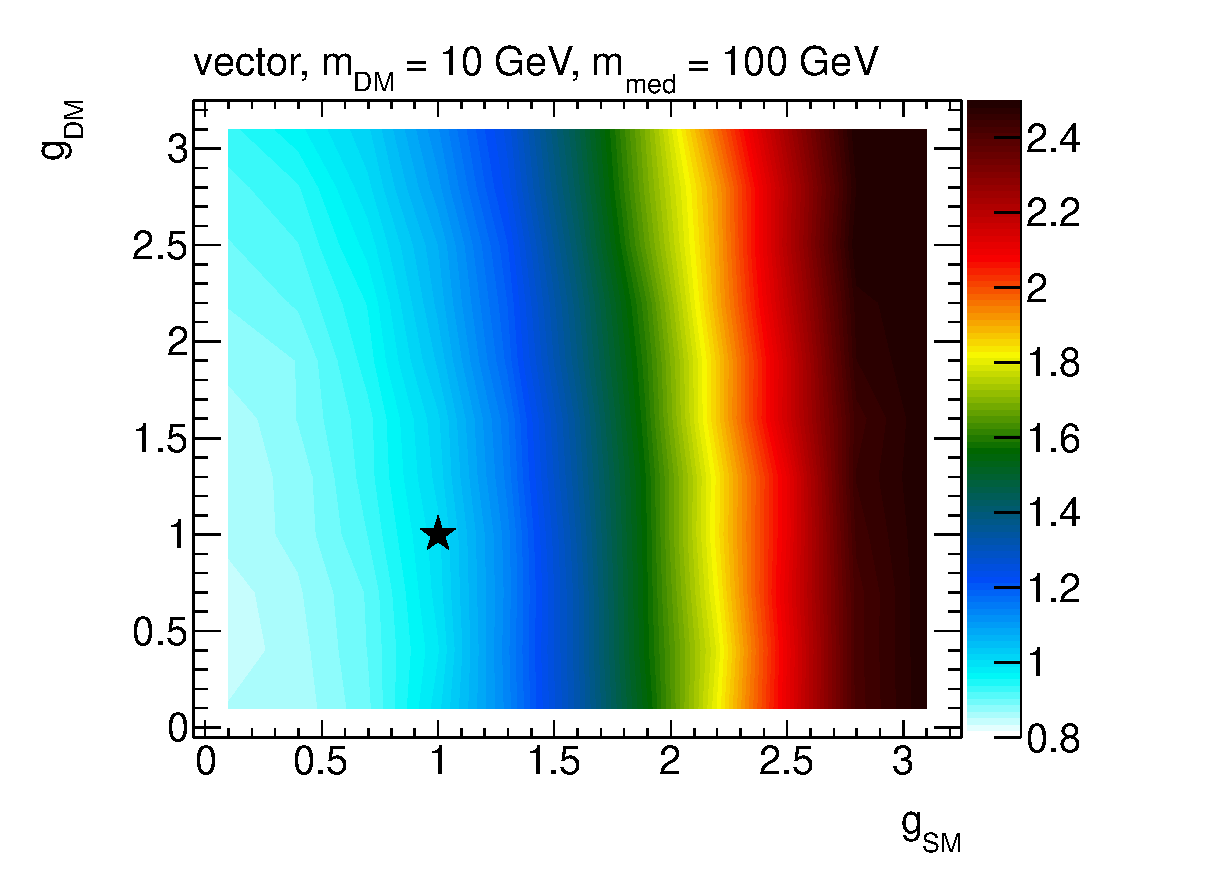
\includegraphics[width=0.45\linewidth]{figures/monojet/scaling_V_10_100.eps}
%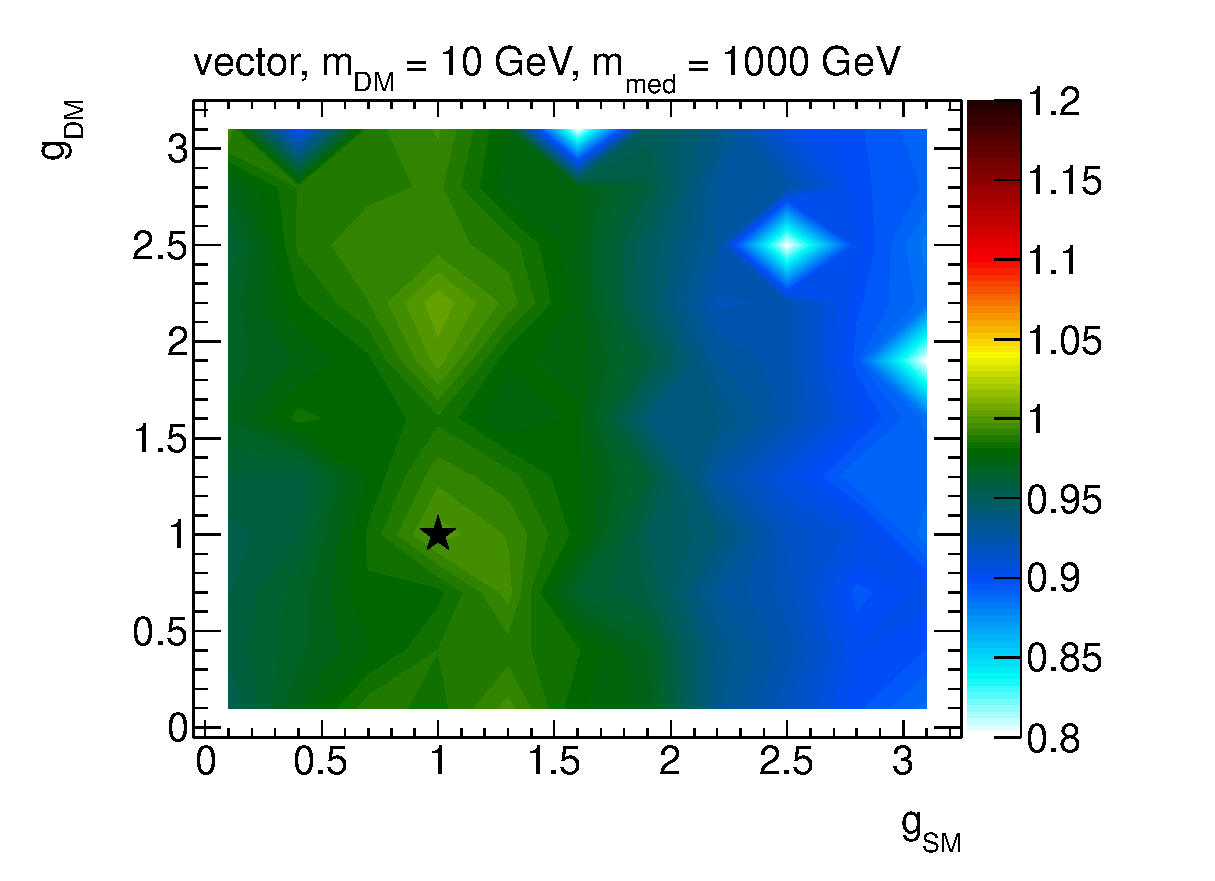
\includegraphics[width=0.45\linewidth]{figures/monojet/scaling_V_10_1000.eps}\\
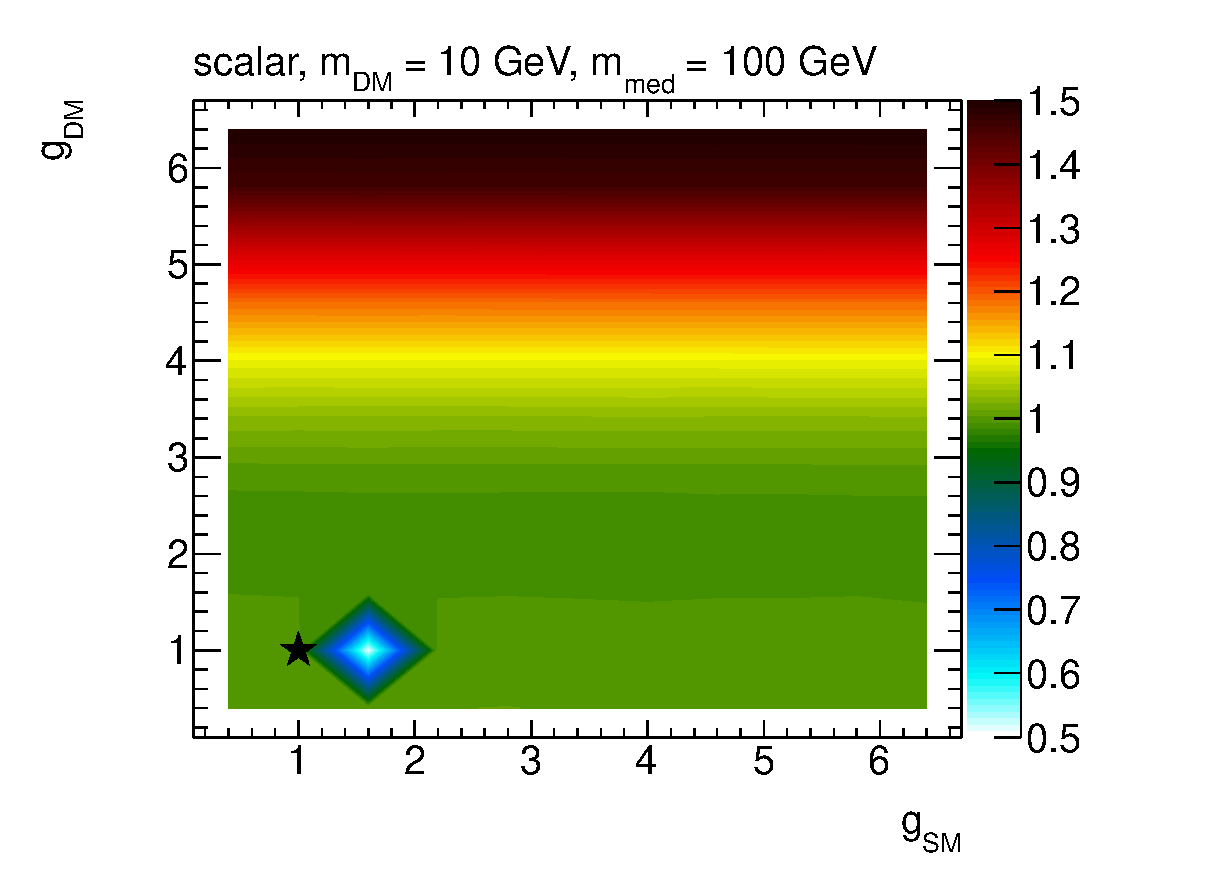
\includegraphics[width=0.45\linewidth]{figures/monojet/scaling_S_10_100.eps}
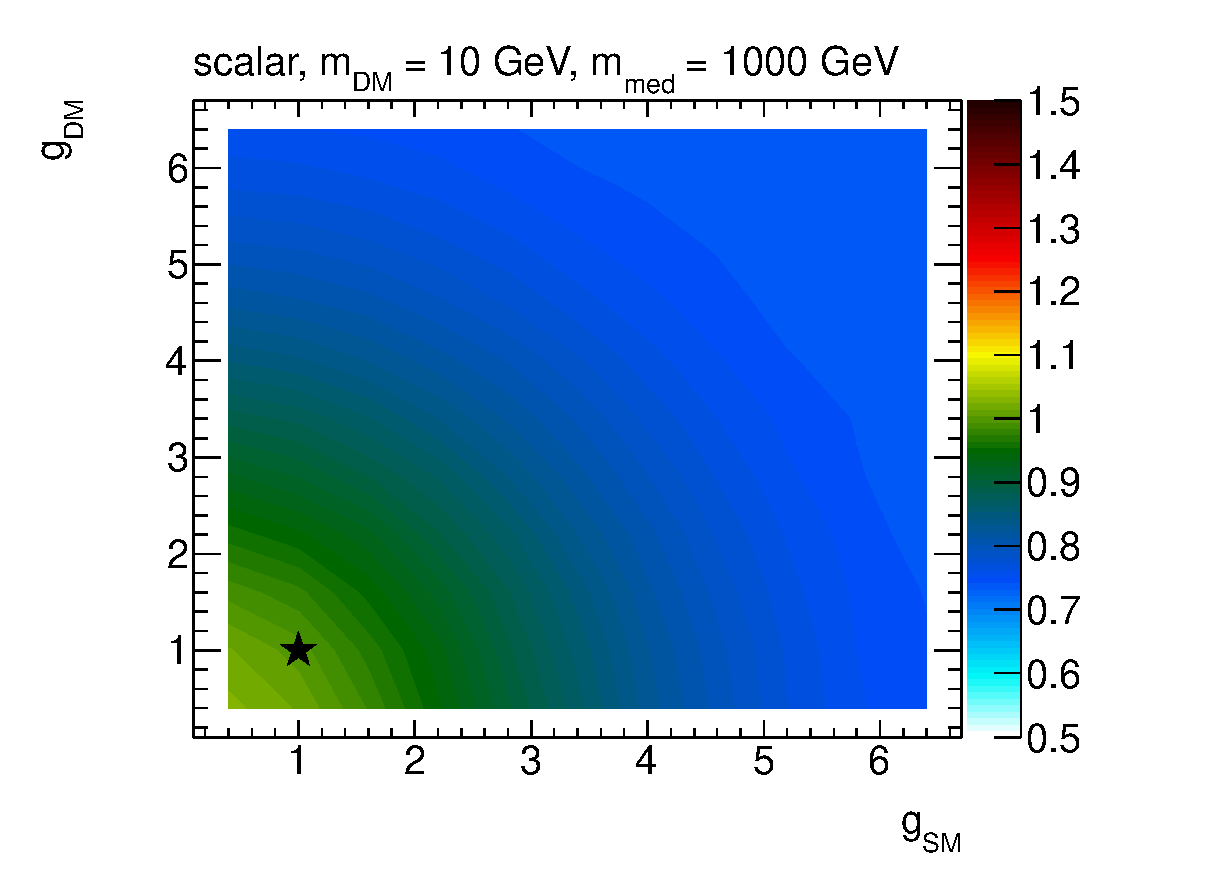
\includegraphics[width=0.45\linewidth]{figures/monojet/scaling_S_10_1000.eps}\\
\caption{Ratio of the rescaled and generated cross sections in the $g_q$--$\gDM$ plane. The point at $g_q=\gDM=1$, taken as a reference for the rescaling, is denoted by a star symbol.
Scalar model with $\mMed=100$\,GeV (left) and 1\,TeV (right) is plotted for $\mDM=10$\,GeV.
The limiting case $\Gamma_{\rm{min}}=\mMed$ is shown as a black line.}
%Vector (scalar) mediator is shown at the top (bottom), the left (right) column corresponds to $\mMed=100$\,GeV ($\mMed=1$\,TeV). Dark Matter mass of 10\,GeV is considered.}
\label{fig:monojet_scaling}
\end{figure}

%The plots are produced with M_S = 300 GeV, m_chi = 100 GeV, gSM = gDM =4
\begin{figure}
\centering
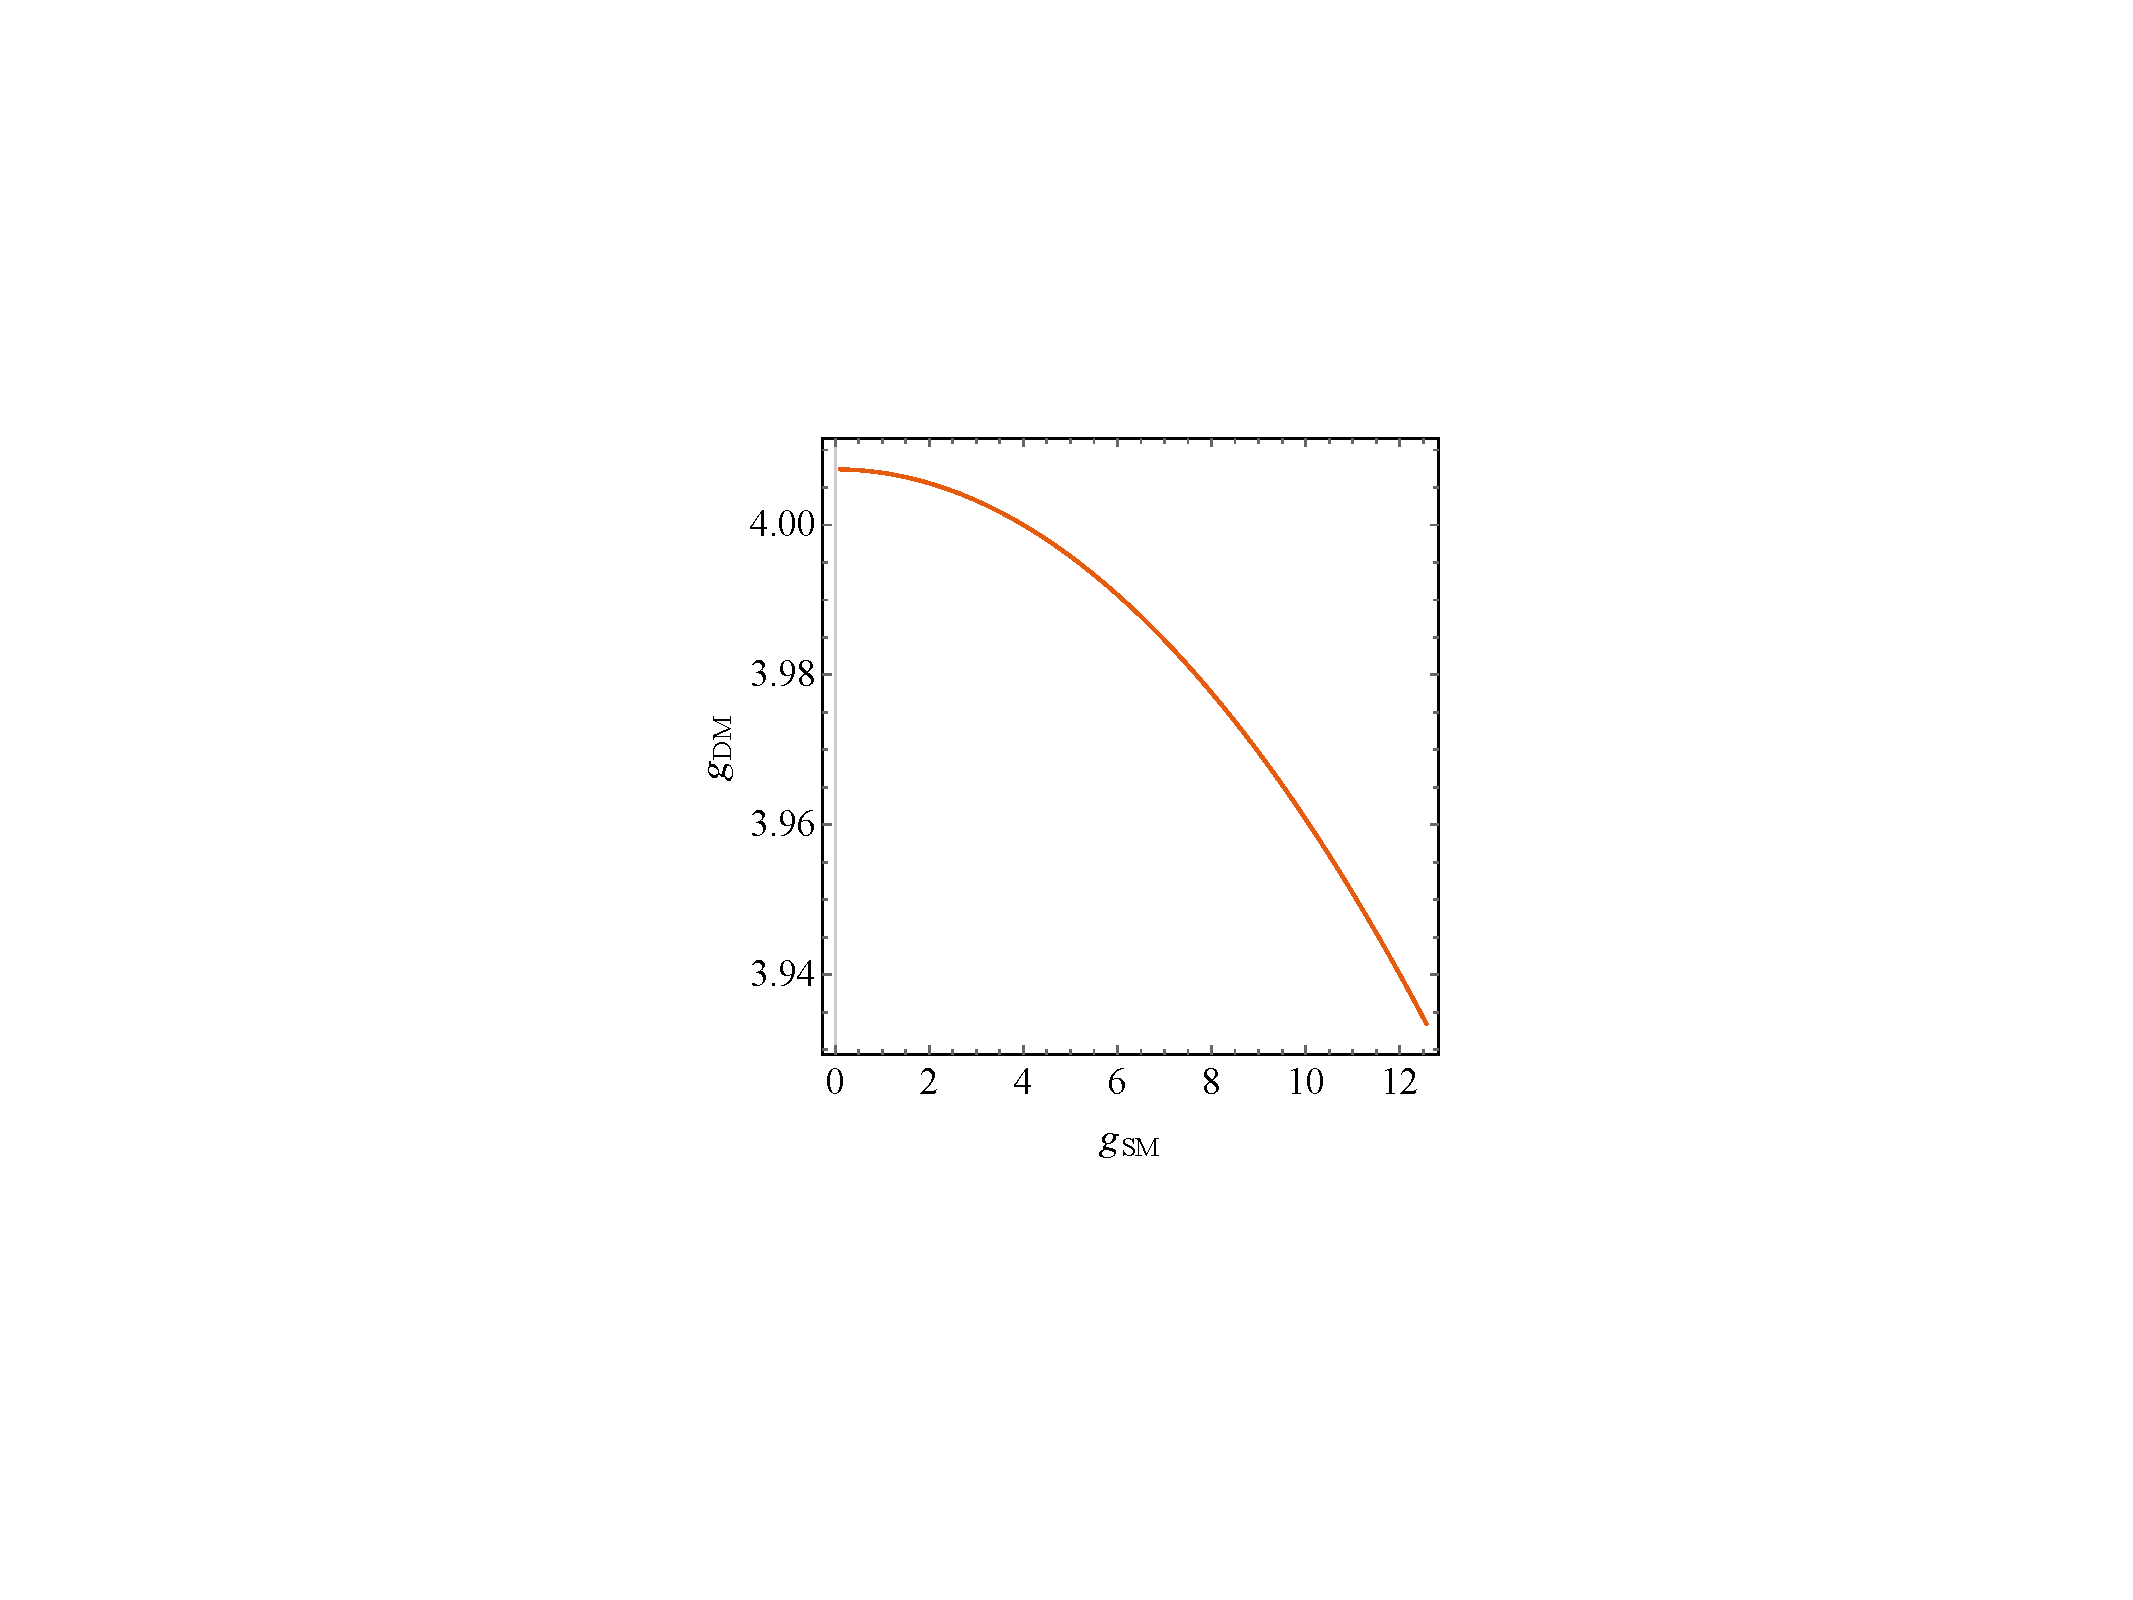
\includegraphics[page=1, trim=310 200 310 200, clip, width=0.3\linewidth]{figures/monojet/rescalingexercise.pdf}
\includegraphics[page=2, trim=305 195 305 195, clip, width=0.3\linewidth]{figures/monojet/rescalingexercise.pdf}
\includegraphics[page=3, trim=300 190 300 190, clip, width=0.3\linewidth]{figures/monojet/rescalingexercise.pdf}
\caption{Scaling along the lines of constant width. The line of constant width for $\mMed=300$\,GeV and $\mDM=100$\,GeV, intercepting $g_q=\gDM=4$ is shown on left. The generated and rescaled cross sections are compared in the middle, the corresponding ratio is shown on right.}
%TODO ask Uli for the color code
\label{fig:monojet_scaling_constwidth}
\end{figure}


\paragraph{Proposed parameter grid}

We propose to present the results in the $g_q$--$\gDM$ plane using the following prescription:
\begin{itemize}
\item Since the shapes of kinematic quantities do not change for different couplings, use the acceptance and efficiency for the available $\mDM=50$\,GeV, $\mMed=300$\,GeV, $g_q=\gDM=1$ grid point from the $\mMed$--$\mDM$ plane for the scalar and pseudo-scalar mediator. In case of the vector and axial-vector mediator, use the grid point $\mDM=50$\,GeV, $\mMed=1$\,TeV, $g_q=\gDM=1$.
\item Generate additional samples in order to get generator cross sections only. For scalar and pseudo-scalar mediator, choose $\mDM=50$\,GeV, $\mMed=300$\,GeV with the following values for $g_q=\gDM$: 0.1, 2, 3, 4, 5, 6. For vector and axial vector mediator, choose $\mDM=50$\,GeV, $\mMed=1$\,TeV with the following values for $g_q=\gDM$: 0.1, 0.25, 0.5, 0.75, 1.25, 1.5. The upper values are defined by the minimal width reaching the mediator mass.
\item Rescale the generator cross sections along the lines of constant width in order to populate the whole $g_q$--$\gDM$ plane.
\end{itemize}

%choose mDM=50, mMed=300, gSM=0.1, gDM={0.1, 1, 2, 3, 4, 5, 6} for S (mMed=GammaMin is reached around 5)
%choose mDM=50, mMed=300, gDM=0.1, gSM={0.1, 0.4, 0.7, 1, 1.3, 1.6, 1.9} for V (mMed=GammaMin is reached around 1.6)
%choose mDM=50, mMed=1000, gDM=0.1, gSM={0.1, 0.4, 0.7, 1, 1.3, 1.6, 1.9} for V (mMed=GammaMin is reached around 1.5)

%choose mDM=50, mMed=300, gSM=gDM={0.1, 1, 2, 3, 4, 5, 6} for S (mMed=GammaMin is reached around 5)
%choose mDM=50, mMed=300, gDM=gSM={0.1, 0.25, 0.5, 0.75, 1, 1.25, 1.5} for V (mMed=GammaMin is reached around 1.5)
%choose mDM=50, mMed=1000, gDM=gSM={0.1, 0.25, 0.5, 0.75, 1, 1.25, 1.5} for V (mMed=GammaMin is reached around 1.4)

\paragraph{Rescaling to different mediator width}

In general there may be an interest to consider larger mediator masses than $\Gamma_{\rm{min}}$ in order to accommodate further couplings of the mediator. The cross section scaling method described above can be used to reinterpret the results presented for the minimal width, since multiplying the width by factor $n$ is equivalent to changing the coupling strength by factor $\sqrt{n}$, i.e.
\begin{equation}
\sigma(g_q,\gDM, n\Gamma_{\rm{min}}(g_q,\gDM)) \propto \frac{g_q^2 \gDM^2}{\Gamma_{\rm{min}}(\sqrt{n}g_q,\sqrt{n}\gDM)} \;.
\end{equation}
The cross section for the sample with couplings $g_q$ and $\gDM$ and modified mediator width $\Gamma = n\Gamma_{\rm{min}}$ can therefore be rescaled from a sample generated with the minimal width corresponding to the couplings scaled by $\sqrt{n}$ as described in the following formula.
\begin{equation}
\sigma(g_q,\gDM, n\Gamma_{\rm{min}}(g_q,\gDM)) = \frac{1}{n^2} \sigma(\sqrt{n}g_q,\sqrt{n}\gDM,\Gamma_{\rm{min}}(\sqrt{n}g_q,\sqrt{n}\gDM))
\end{equation}
Advantage of doing this is again in the fact that no event selection and detector response needs to be simulated since the changes in couplings do not have an effect on the shapes of kinematic distributions.




\subsection{POWHEG settings}

This section describes specif settings for the Dark Matter models needed to run the POWHEG generation.
\begin{itemize}
\item The POWHEG implementation allows to generate a single sample that provides sufficient statistics in all mono-jet analysis signal regions. %by optimizing the following two parameters:
%\begin{itemize}
POWHEG generates weighted events and the \verb+bornsuppfact+ parameter is used to set the event suppression factor according to
\begin{equation}
F(k_{\rm{T}})=\frac{k_{\rm{T}}^2}{k_{\rm{T}}^2+\texttt{bornsuppfact}^2} \;.
\end{equation}
In this way, the events at low $\MET$ are suppressed and receive higher event weights which ensures higher statistics at high $\MET$. We recommend to set \verb+bornsuppfact+ to 1000.
\item The \verb+bornktmin+ parameter allows to suppress the low $\MET$ region even further by starting the generation at a certain value of $k_{\rm{T}}$. It is recommended to set this parameter  to half the lower analysis $\MET$ cut, therefore the proposed value for \verb+bornktmin+ is 150.
%\end{itemize}

\item Set \verb+runningwidth+ to 0.
\item Set \verb+mass_low+ and \verb+mass_high+ to -1.
\item The minimal values for \verb+ncall1+, \verb+itmx1+, \verb+ncall2+, \verb+itmx2+ are 250000, 5, 1000000, 5 for the DMV model, respectively. In order to increase speed, set \verb+foldsci+ and \verb+foldy+ to 2 and keep \verb+foldphi+ at 1. 
\item The minimal values for \verb+ncall1+, \verb+itmx1+, \verb+ncall2+, \verb+itmx2+ are 100000, 5, 100000, 5 for the DMS\_tloop model, respectively.
\item Allow negative weights for the DMV model by setting \verb+withnegweights+ to 1.
\item Since the DMS\_tloop model is a leading order process, set \verb+LOevents+ and \verb+bornonly+ are set to 1 internally.
\end{itemize}


\subsection{Colored scalar mediator, t-channel exchange}

\input tex/TChannelModels.tex

